\documentclass{beamer}
\usepackage[utf8]{inputenc}
\usepackage[dutch]{babel}
\usepackage{keystroke}

\usepackage{hyperref}
% colored links
\hypersetup{
    colorlinks=true,
    linkcolor=blue,
    urlcolor=blue,
}

\usetheme{Madrid}
\usecolortheme{default}

%------------------------------------------------------------
%This block of code defines the information to appear in the
%Title page
\title[Debian installatie] %optional
{Debian installatie met preseed}

% \subtitle{A short story}

\author[S.L.Speek] % (optional)
{Steven L. Speek}

\institute[ACC] % (optional)
{
  Actief Computer Centrum
}

\date[\today{}] % (optional)
{\today{}}

% \logo{\includegraphics[height=1cm]{overleaf-logo}}

%End of title page configuration block
%------------------------------------------------------------



%------------------------------------------------------------
%The next block of commands puts the table of contents at the 
%beginning of each section and highlights the current section:

% \AtBeginSection[]
% {
%   \begin{frame}<handout:0>
%     \frametitle{Inhoudsopgave}
%     \tableofcontents[currentsection]
%   \end{frame}
% }
\newif\iflattersubsect

\AtBeginSection[] {
    \begin{frame}<beamer>
      \frametitle{Inhoudsopgave}
      \tableofcontents[currentsection]
     \end{frame}
    \lattersubsectfalse
}

\AtBeginSubsection[] {
    \iflattersubsect
    \begin{frame}<beamer>
      \frametitle{Inhoudsopgave}
      \tableofcontents[currentsubsection]
    \end{frame}
    \fi
    \lattersubsecttrue
}
%------------------------------------------------------------


\begin{document}

%The next statement creates the title page.
\frame{\titlepage}


%---------------------------------------------------------
%This block of code is for the table of contents after
%the title page
\begin{frame}
\frametitle{Inhoudsopgave}
\tableofcontents
\end{frame}
%---------------------------------------------------------


\section{Installatie media}

%---------------------------------------------------------
\begin{frame}
\frametitle{Installatie media downloaden}
Klik `Downloaden' op \href{https://debian.org}{debian.org}

\centering
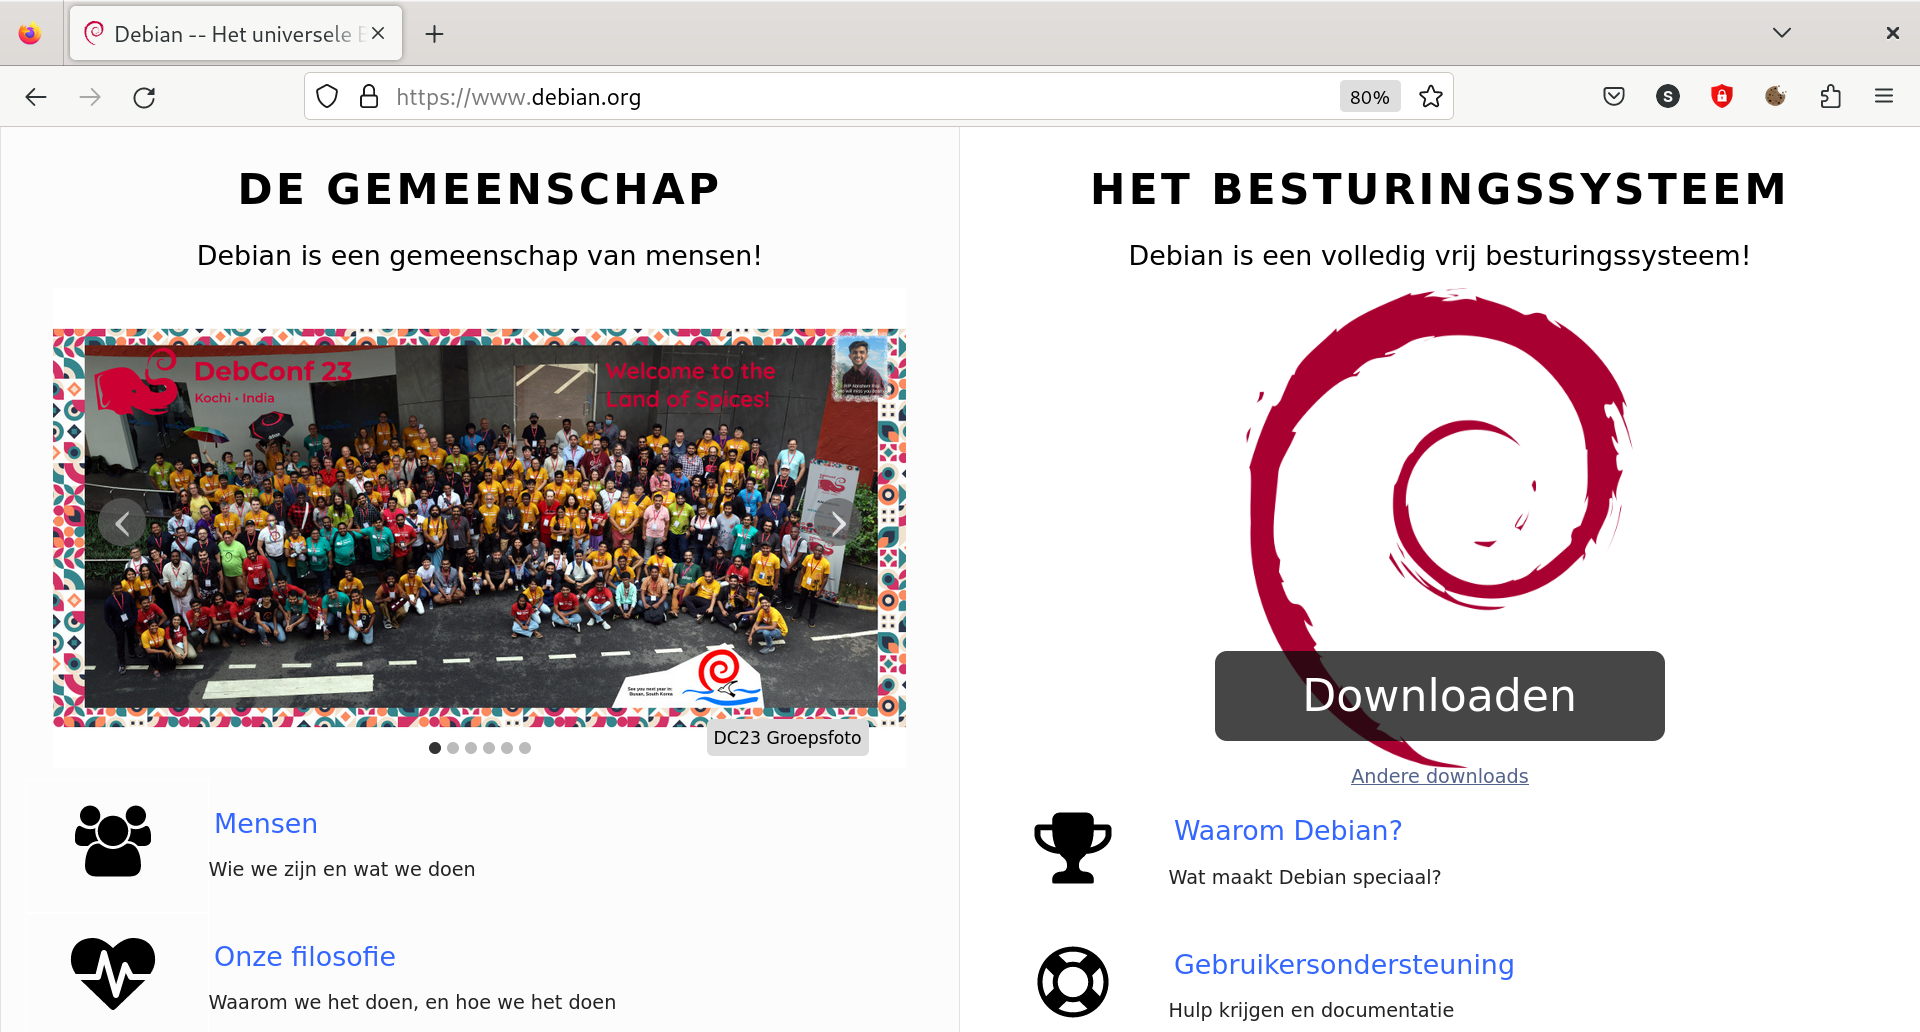
\includegraphics[width=\textwidth]{img/debian-downloaden.png} 
\end{frame}

\begin{frame}
  \frametitle{Installatie USB-stick maken}
\begin{itemize}
    \item Download en installeer \href{https://rufus.ie}{Rufus}
    \item Maak een USB-stick met het debian ISO-image met Rufus
\end{itemize}
\end{frame}

%---------------------------------------------------------


%---------------------------------------------------------
\section{De installer booten}

\begin{frame}
  \frametitle{De \textbf{debian-installer} booten}
  \begin{itemize}
    \item Steek de USB-stick met het debian ISO-image in de computer
    \item Sluit de computer bedraad aan op het netwerk
    \item Zoek \href{https://www.boot-disk.com/quest_bootmenu.htm}{hier} de toets op die op uw computer het \href{https://www.boot-disk.com/quest_bootmenu.htm}{boot menu} toont
    \item Start de computer op en ga het \href{https://www.boot-disk.com/quest_bootmenu.htm}{boot menu} in
    \item Kies de USB-stick met het debian ISO-image
  \end{itemize}

\end{frame}
%---------------------------------------------------------


%---------------------------------------------------------
\begin{frame}
  \frametitle{Installer grub menu}
  \begin{itemize}
    \item<2-> binnen 30 seconden \DArrow indrukken
    \item<3> \DArrow, \UArrow\  en \Enter om deze menu's te bedienen
  \end{itemize}
  
  \centering
  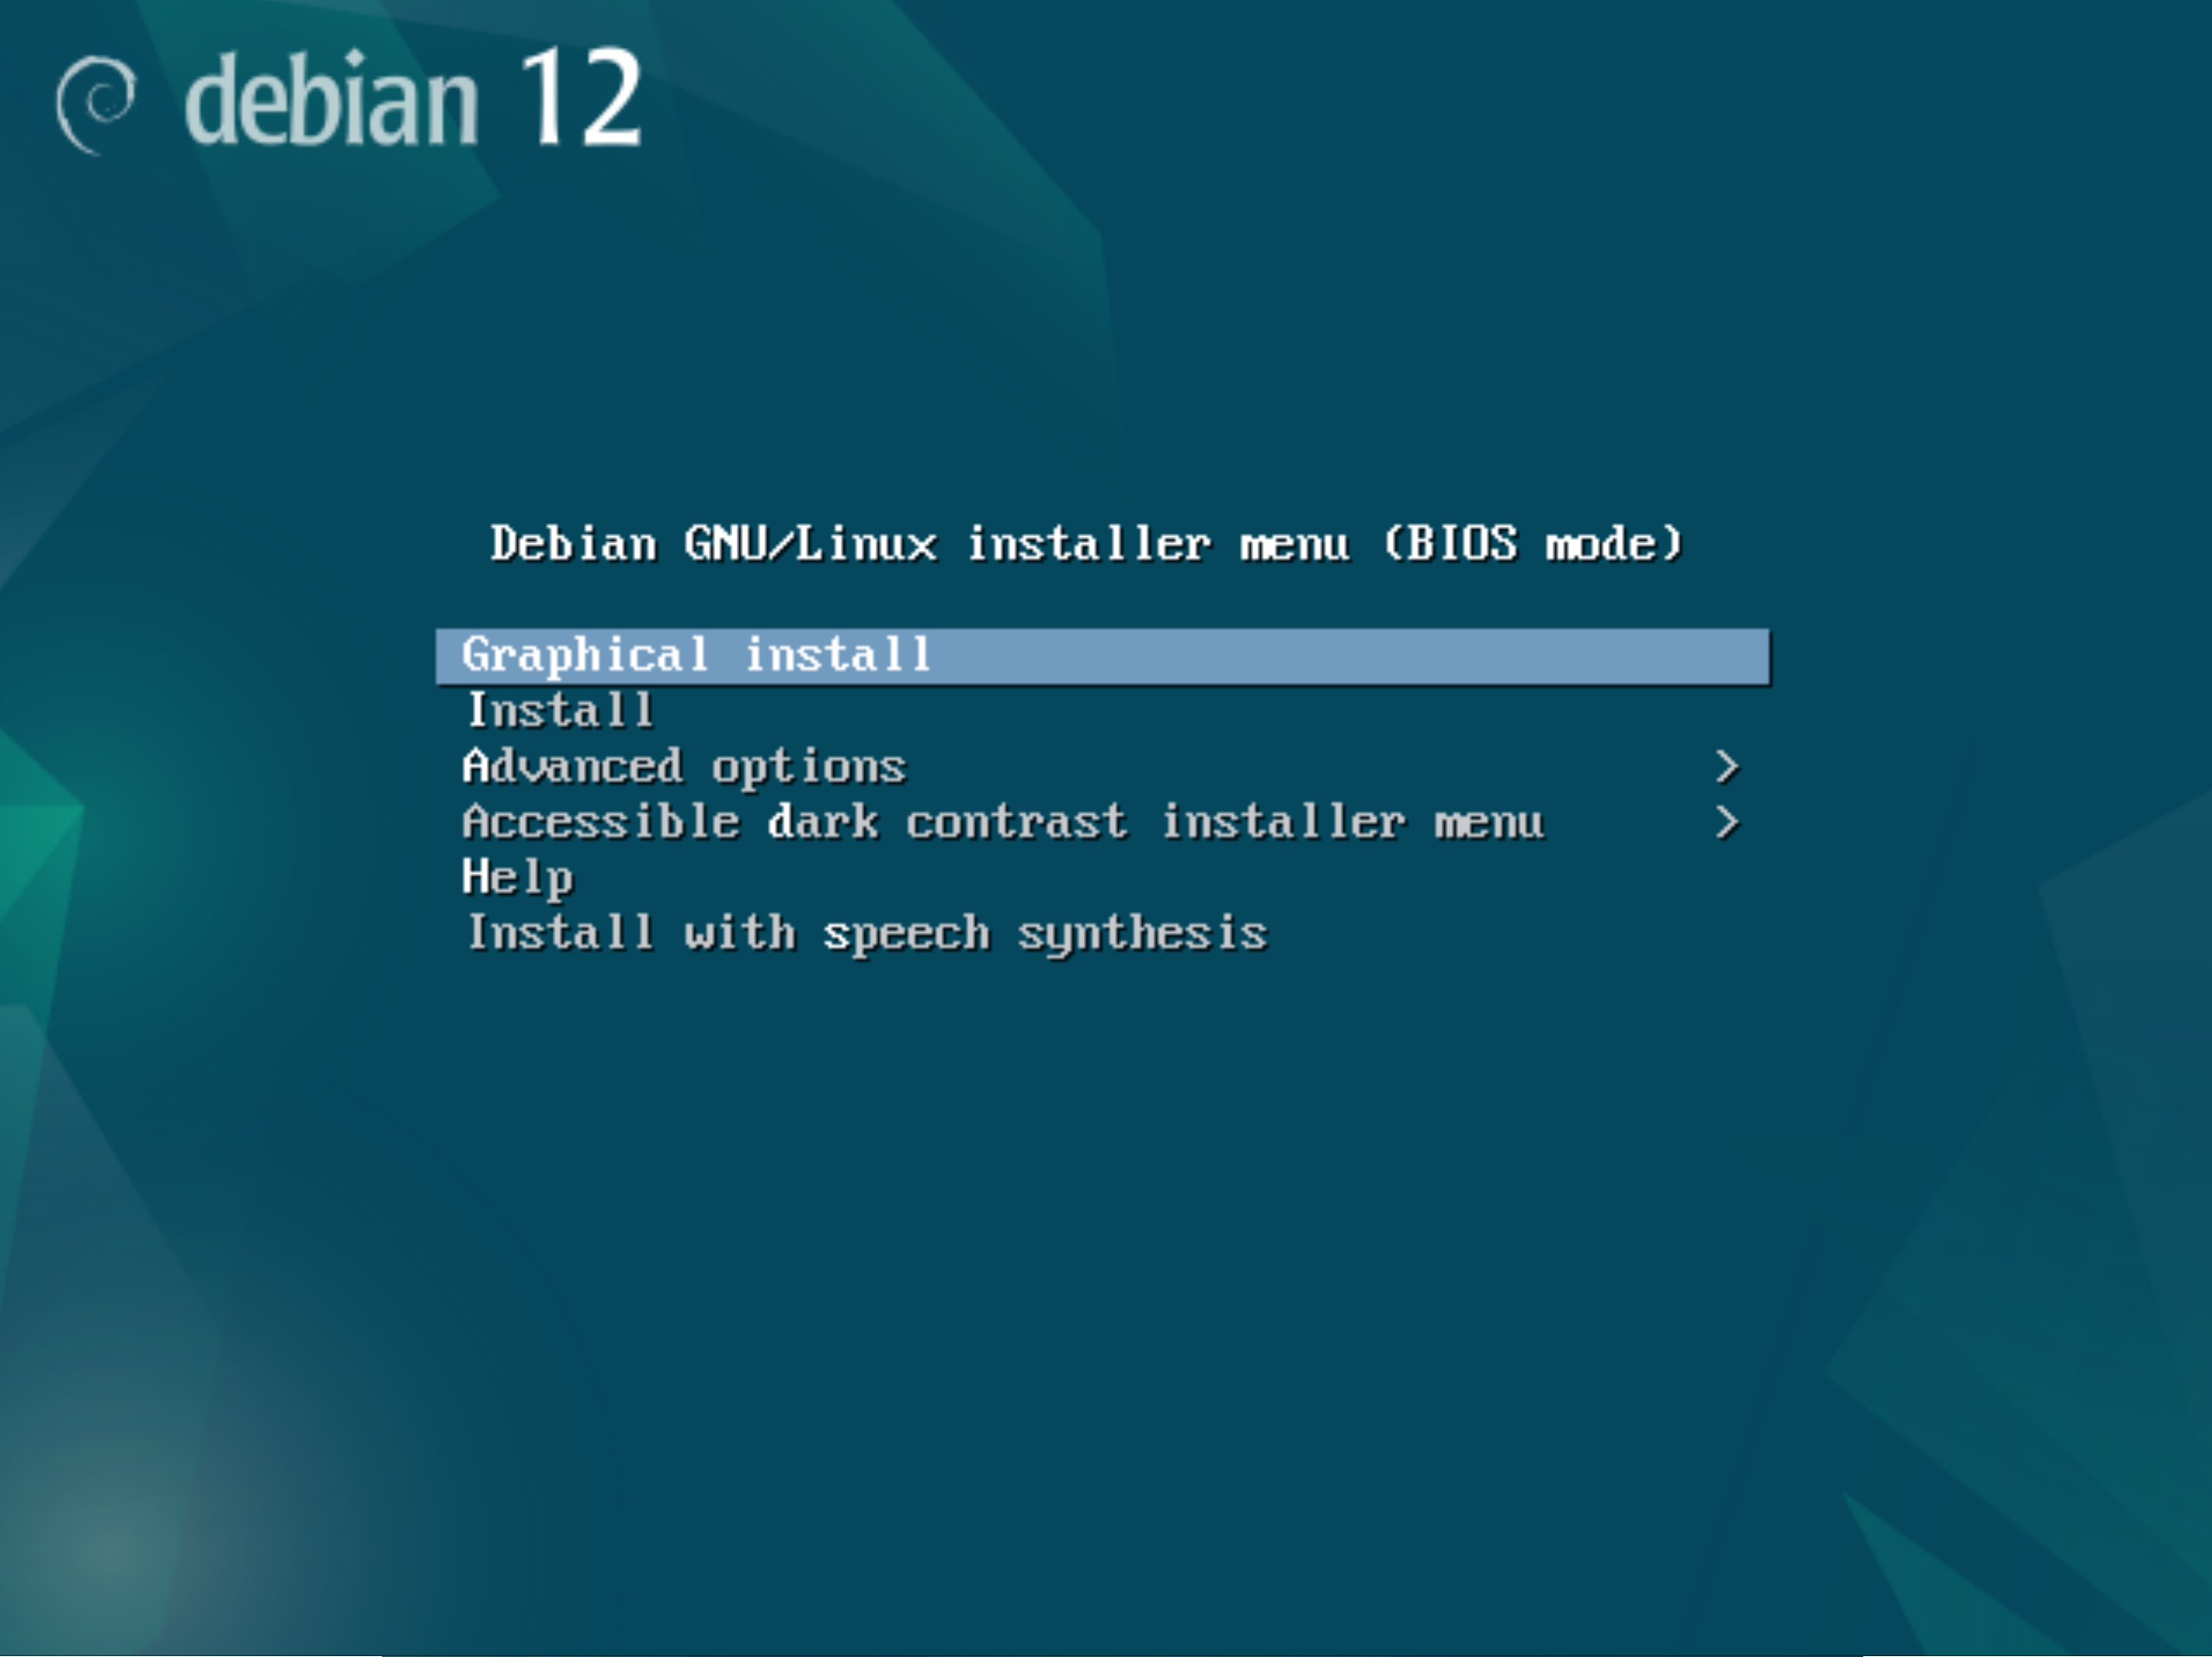
\includegraphics[width=0.8\textwidth]{img/installer-grub-menu.png}<1->
\end{frame}

\section{Automatische installatie}

\begin{frame}
  \frametitle{Geavanceerde installatie kiezen}
  \onslide<2>{2 keer \DArrow en \Enter}
  \centering
  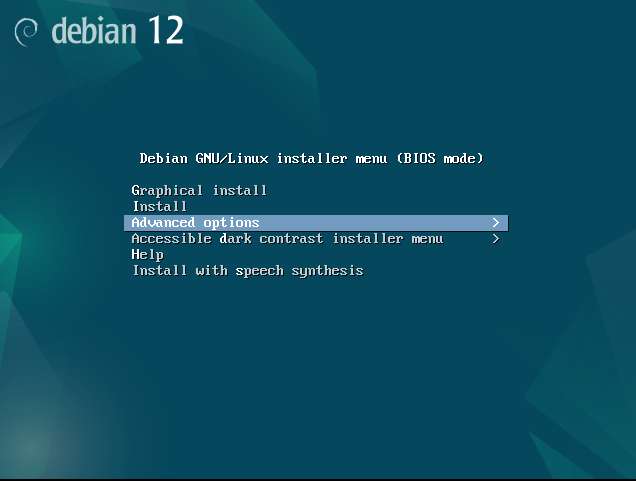
\includegraphics[width=\textwidth]{img/advanced-options.png}<1->
\end{frame}

\begin{frame}
  \frametitle{Automatische installatie kiezen}
  \onslide<2>{6 keer \DArrow en \Enter}
  \centering
  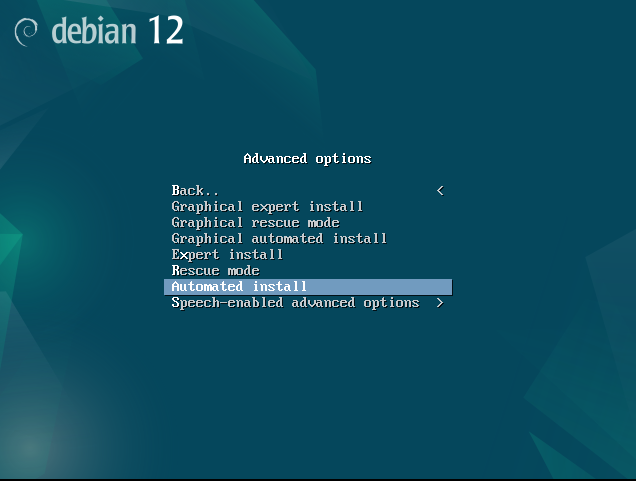
\includegraphics[width=\textwidth]{img/automated-install.png}<1->
\end{frame}

\begin{frame}
   \frametitle{Bedienen van de debian installer}
   \begin{itemize}
      \item \Tab{} en \RArrow{} om verder te gaan
      \item \Shift{}+\Tab{} en \LArrow{} om terug te gaan
      \item \UArrow{}, \DArrow{}, \PgUp{}, en \PgDown om in lijsten te navigeren
      % \item \Spacebar om checkboxen te selecten of deselecteren
      \item \Enter om te kiezen
   \end{itemize}
\end{frame}

\subsection{Netwerk}

\begin{frame}
   \frametitle{Netwerk interface kiezen}
   Indien de computer ook wifi heeft moet een keuze worden gemaakt voor de bedraade netwerk aansluiting
\end{frame}

\subsection{Preseed}
\begin{frame}
   \frametitle{Wat is preseeding?}
   \begin{itemize}
      \item Preseeding beantwoord met behulp van een preconfiguation bestand vragen van de debian-installer
      \item Voorbeeld \href{https://www.debian.org/releases/stable/example-preseed.txt}{https://www.debian.org/releases/stable/example-preseed.txt}
      \item Meer info op \href{https://wiki.debian.org/DebianInstaller/Preseed}{https://wiki.debian.org/DebianInstaller/Preseed}
   \end{itemize}


\end{frame}

\begin{frame}
   \frametitle{Preconfiguration file}
   U voert \texttt{https://slspeek.github.io/debian/gnome-complete.cfg} in
   
   \centering
   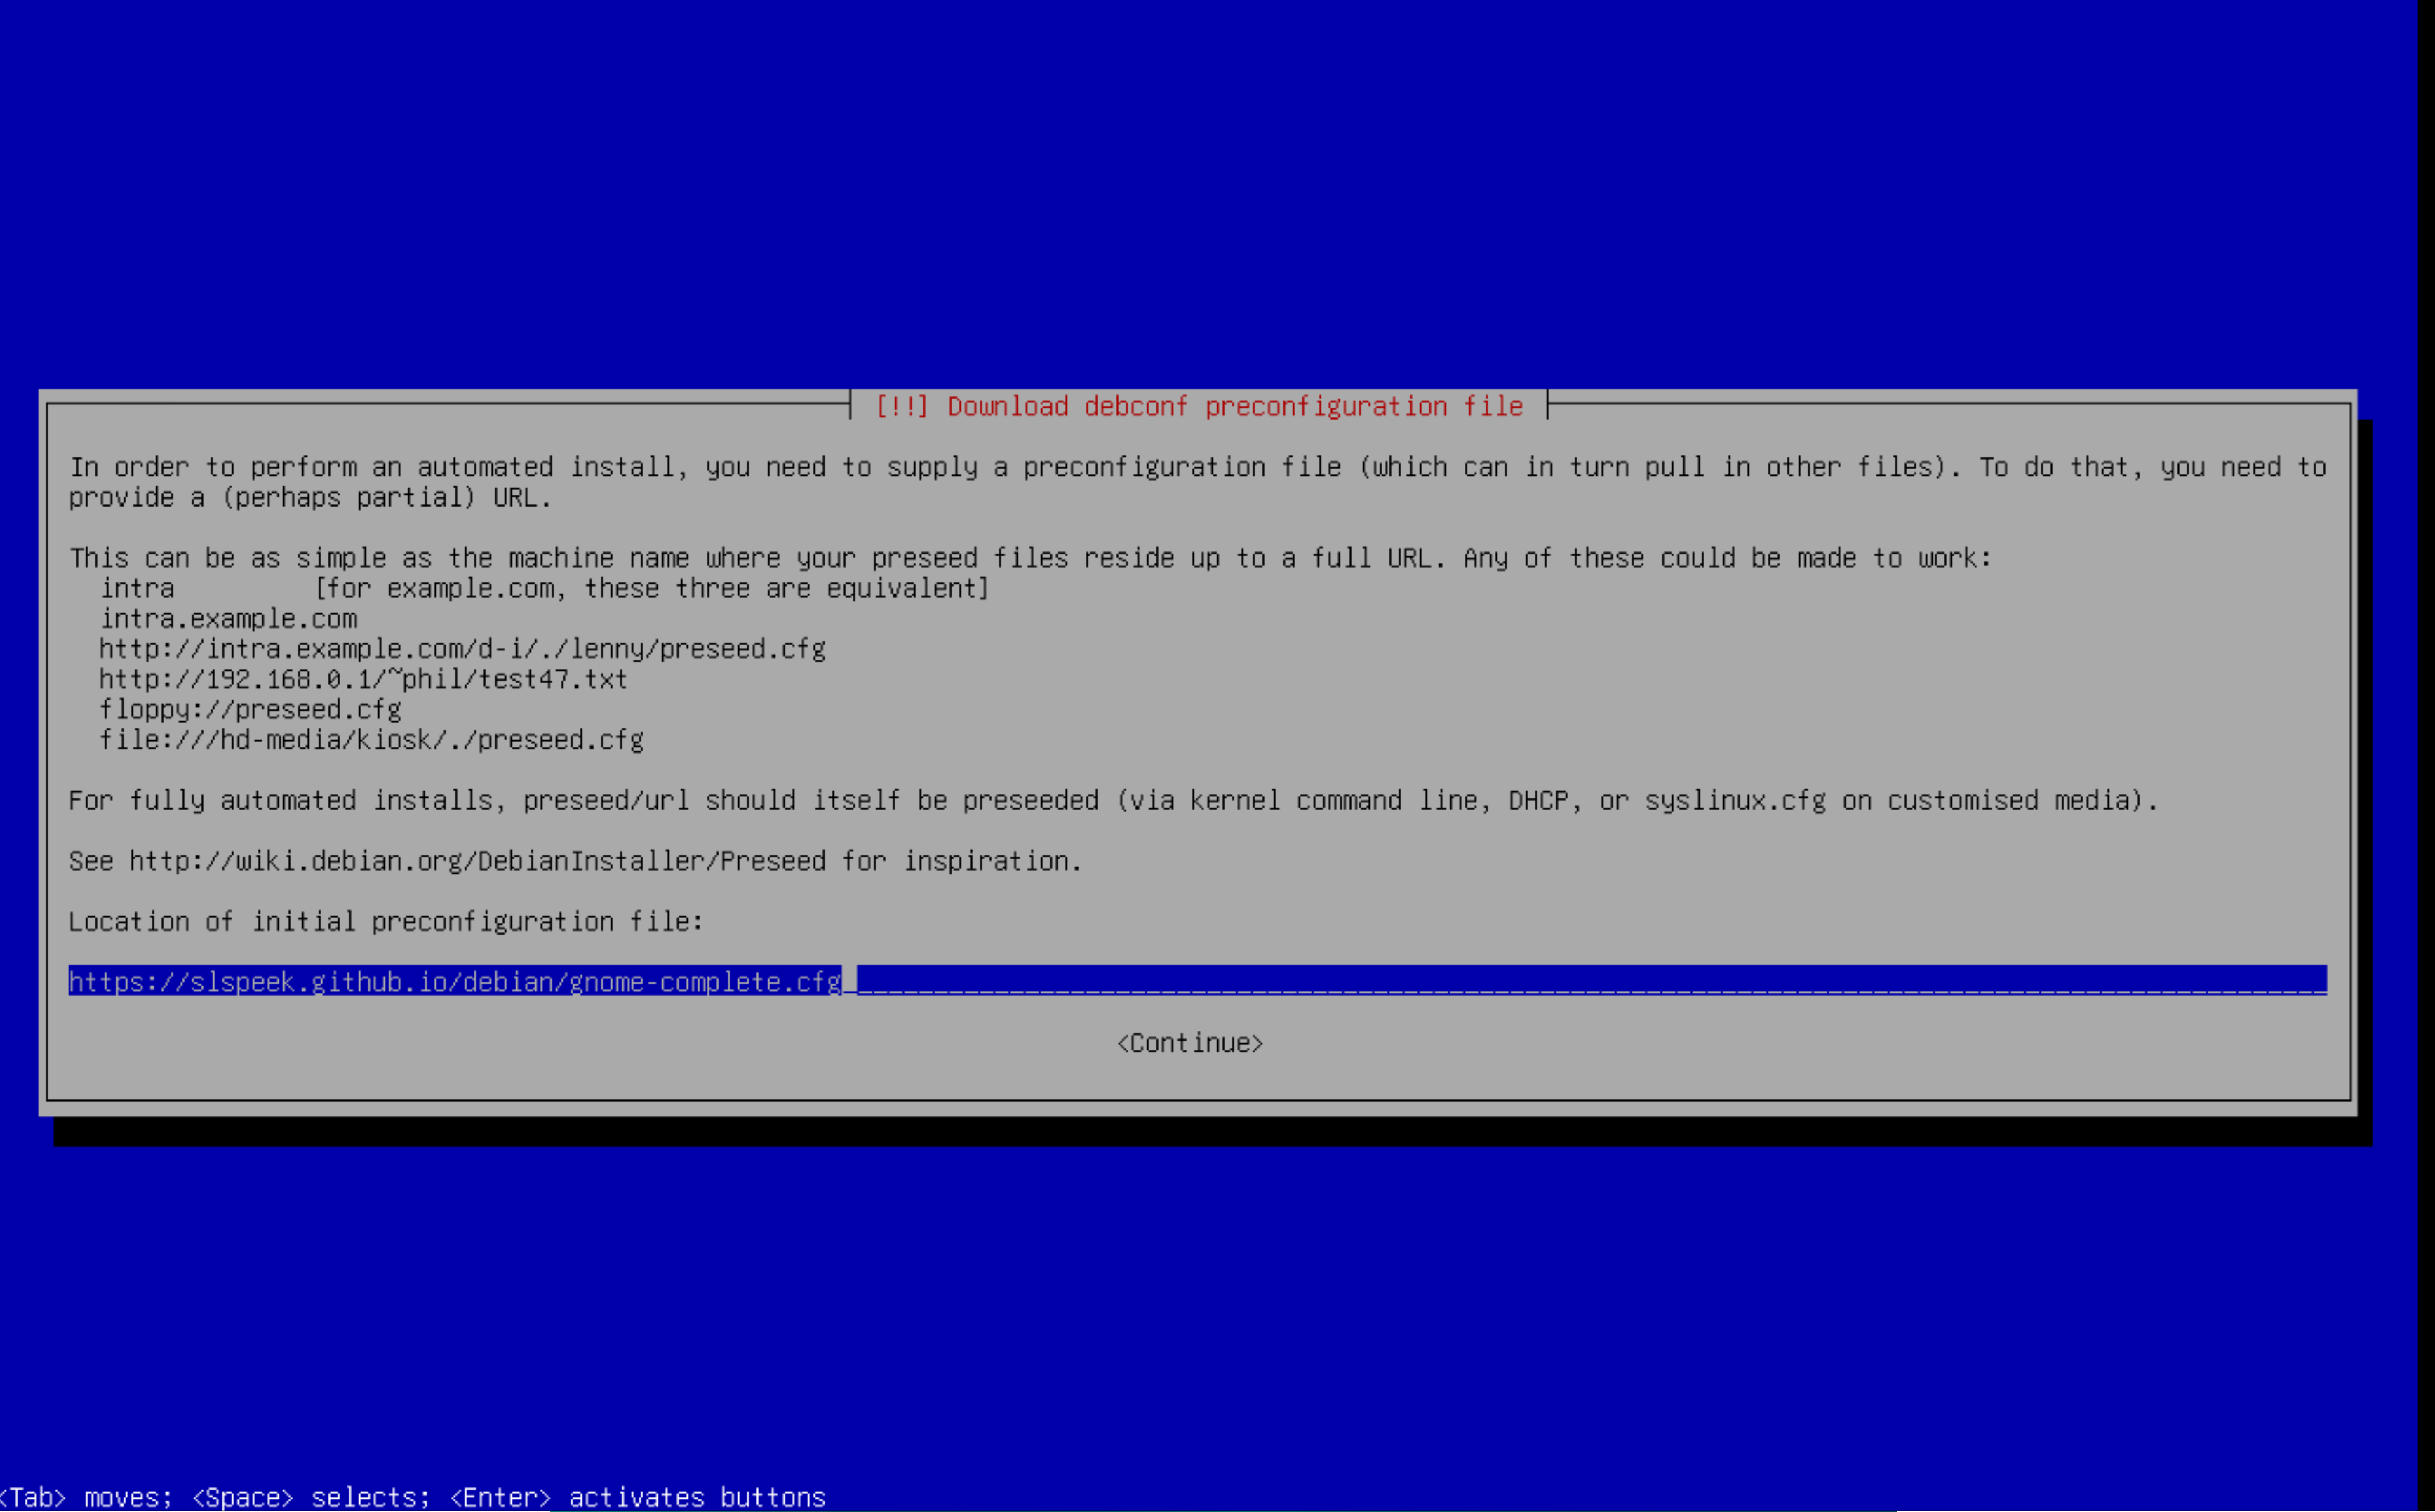
\includegraphics[width=0.8\textwidth]{img/preseed-adres.png}
\end{frame}

\begin{frame}
   \frametitle{Alternatieve configuraties}
   Op \href{https://slspeek.github.io/debian/}{Nederlandse Debian preseeds} vindt u meer configuraties:
   \begin{itemize}
      \item \textbf{Personal} varianten waarbij u in de installer een gebruiker kunt opgeven (ipv tux)
      \item Niet \textbf{complete} varianten met minder ge\"{i}nstalleerde pakketen
      \item Andere desktop varianten \begin{itemize}
         \item MATE
         \item LXDE
      \end{itemize}

   \end{itemize}

\end{frame}

\subsection{Disk indeling}
\begin{frame}
   \frametitle{Gehele disk kiezen}
   \onslide<2>{\Enter op om door te gaan}
   \centering
   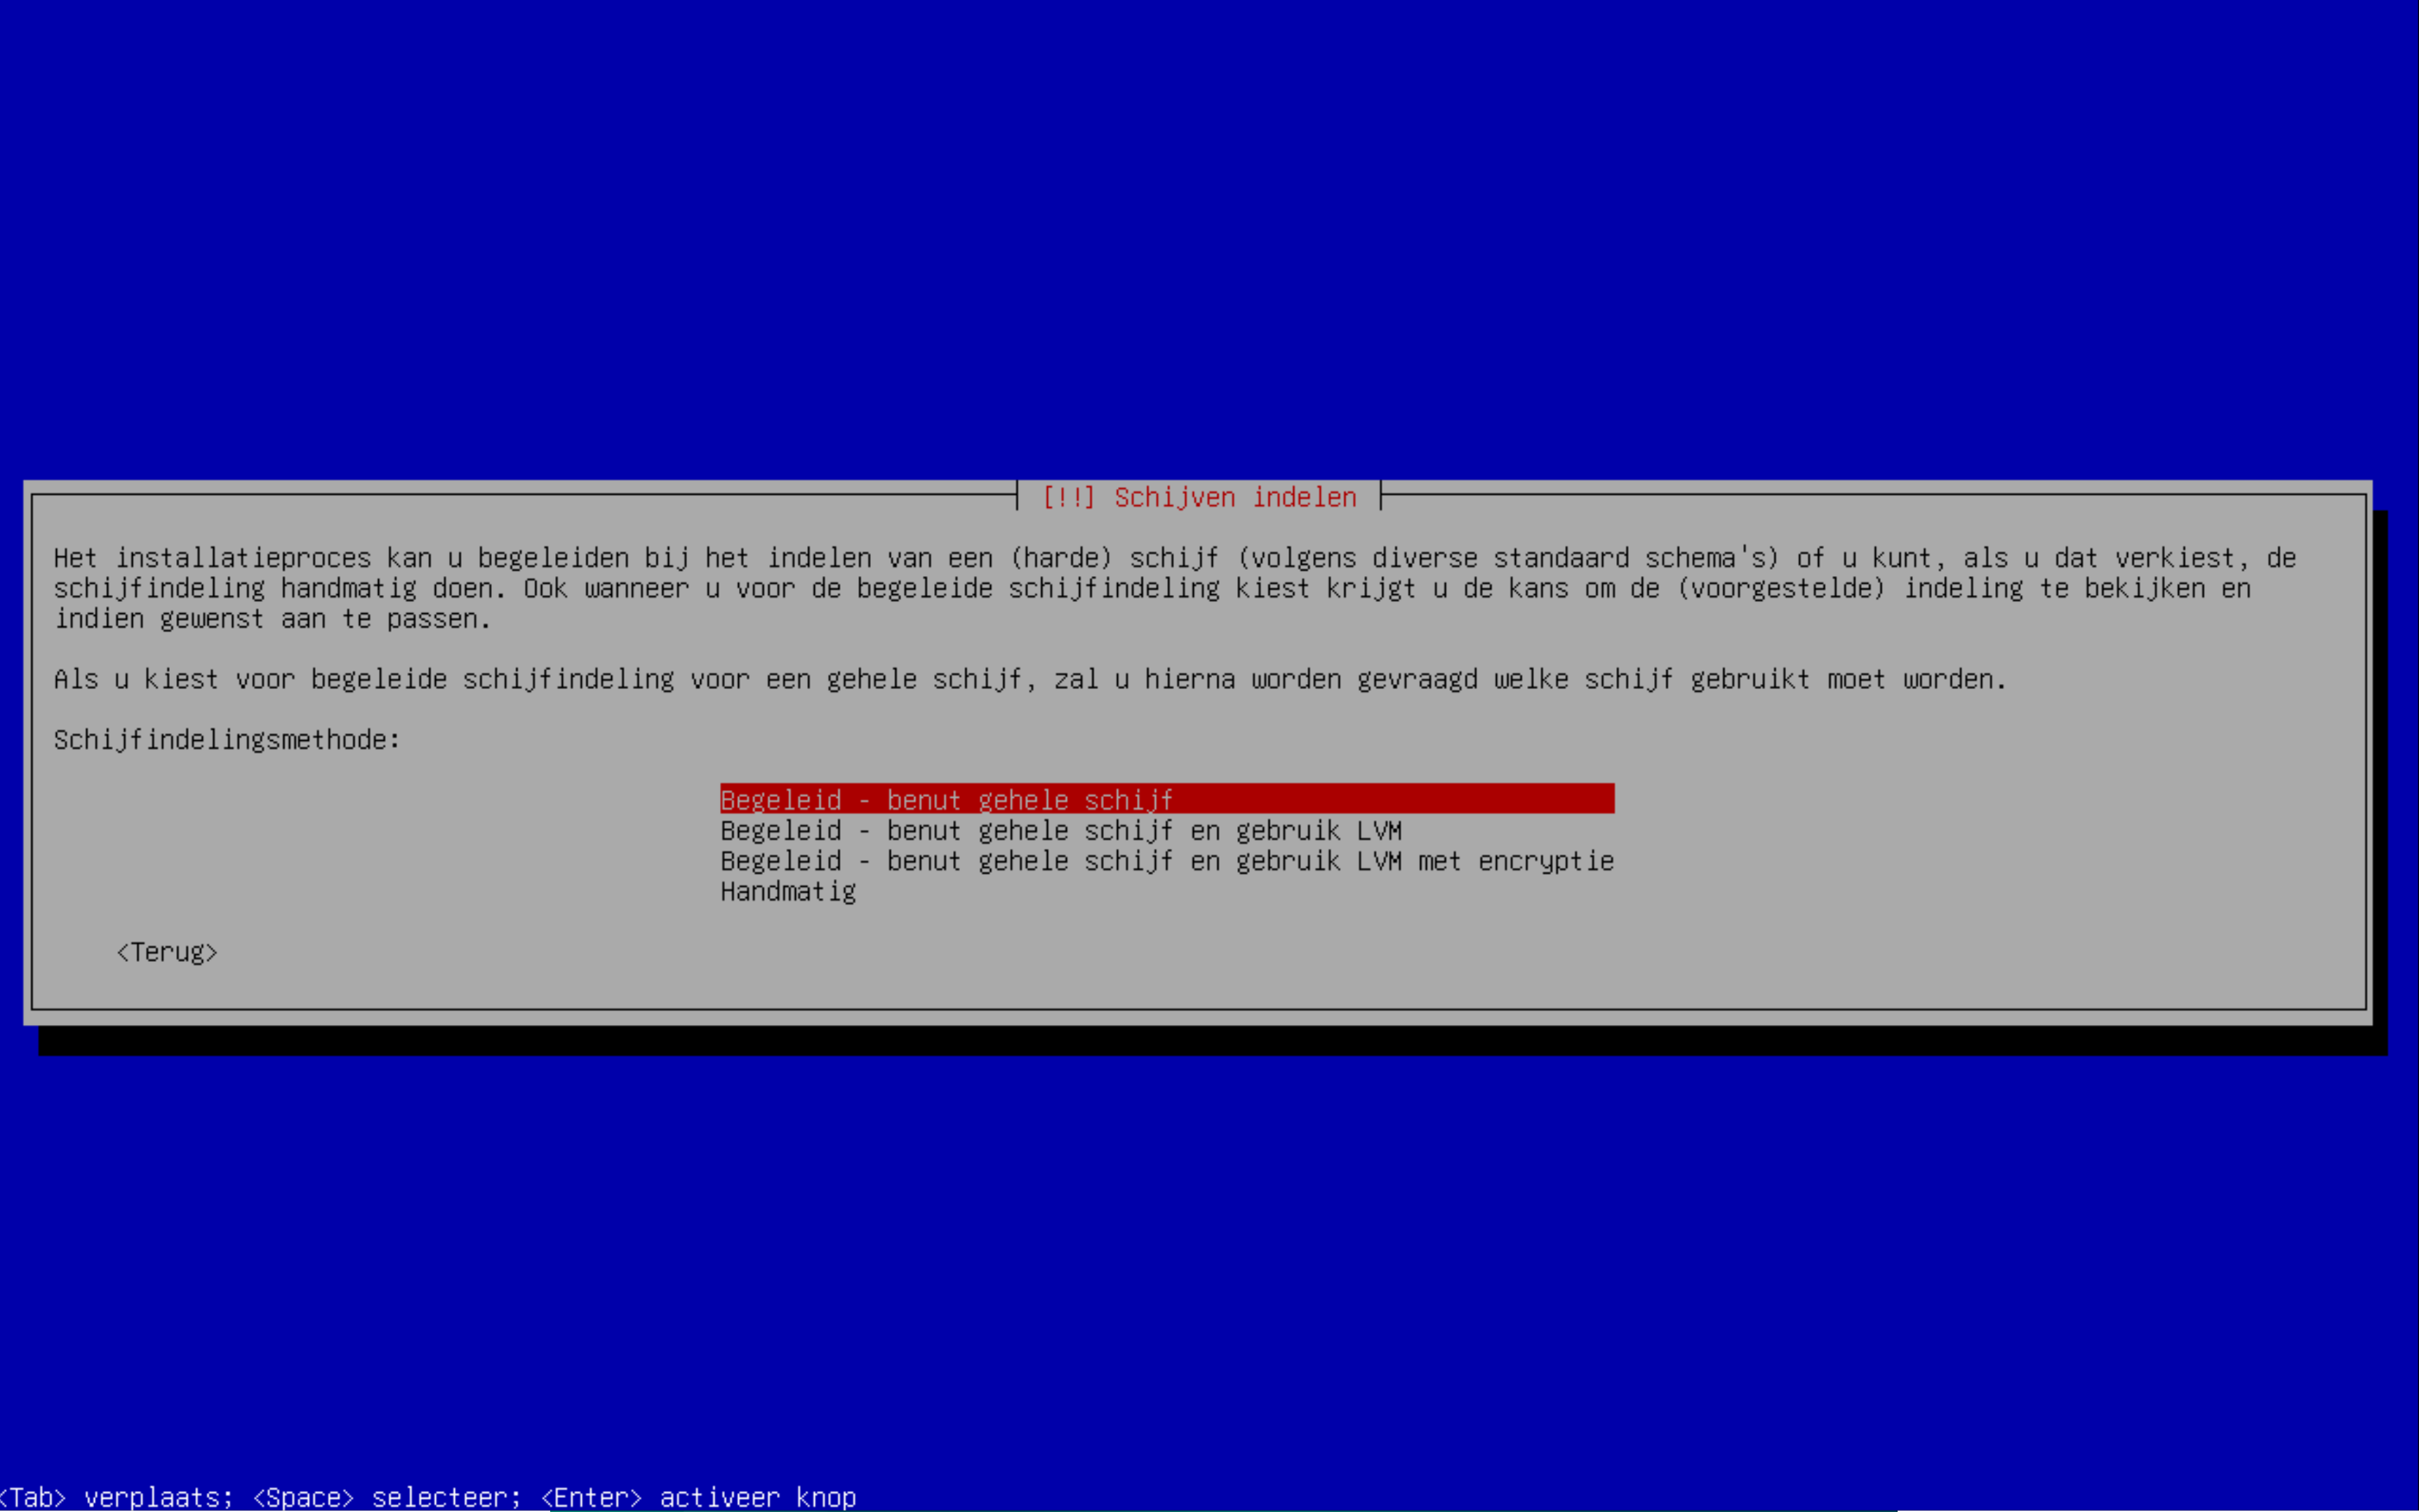
\includegraphics[width=\textwidth]{img/gehele-disk-kiezen.png}<1->
\end{frame}

\begin{frame}
  \frametitle{Disk kiezen}
  \onslide<2>{Kies met \UArrow en \DArrow een disk en bevestig met \Enter}
  \centering
  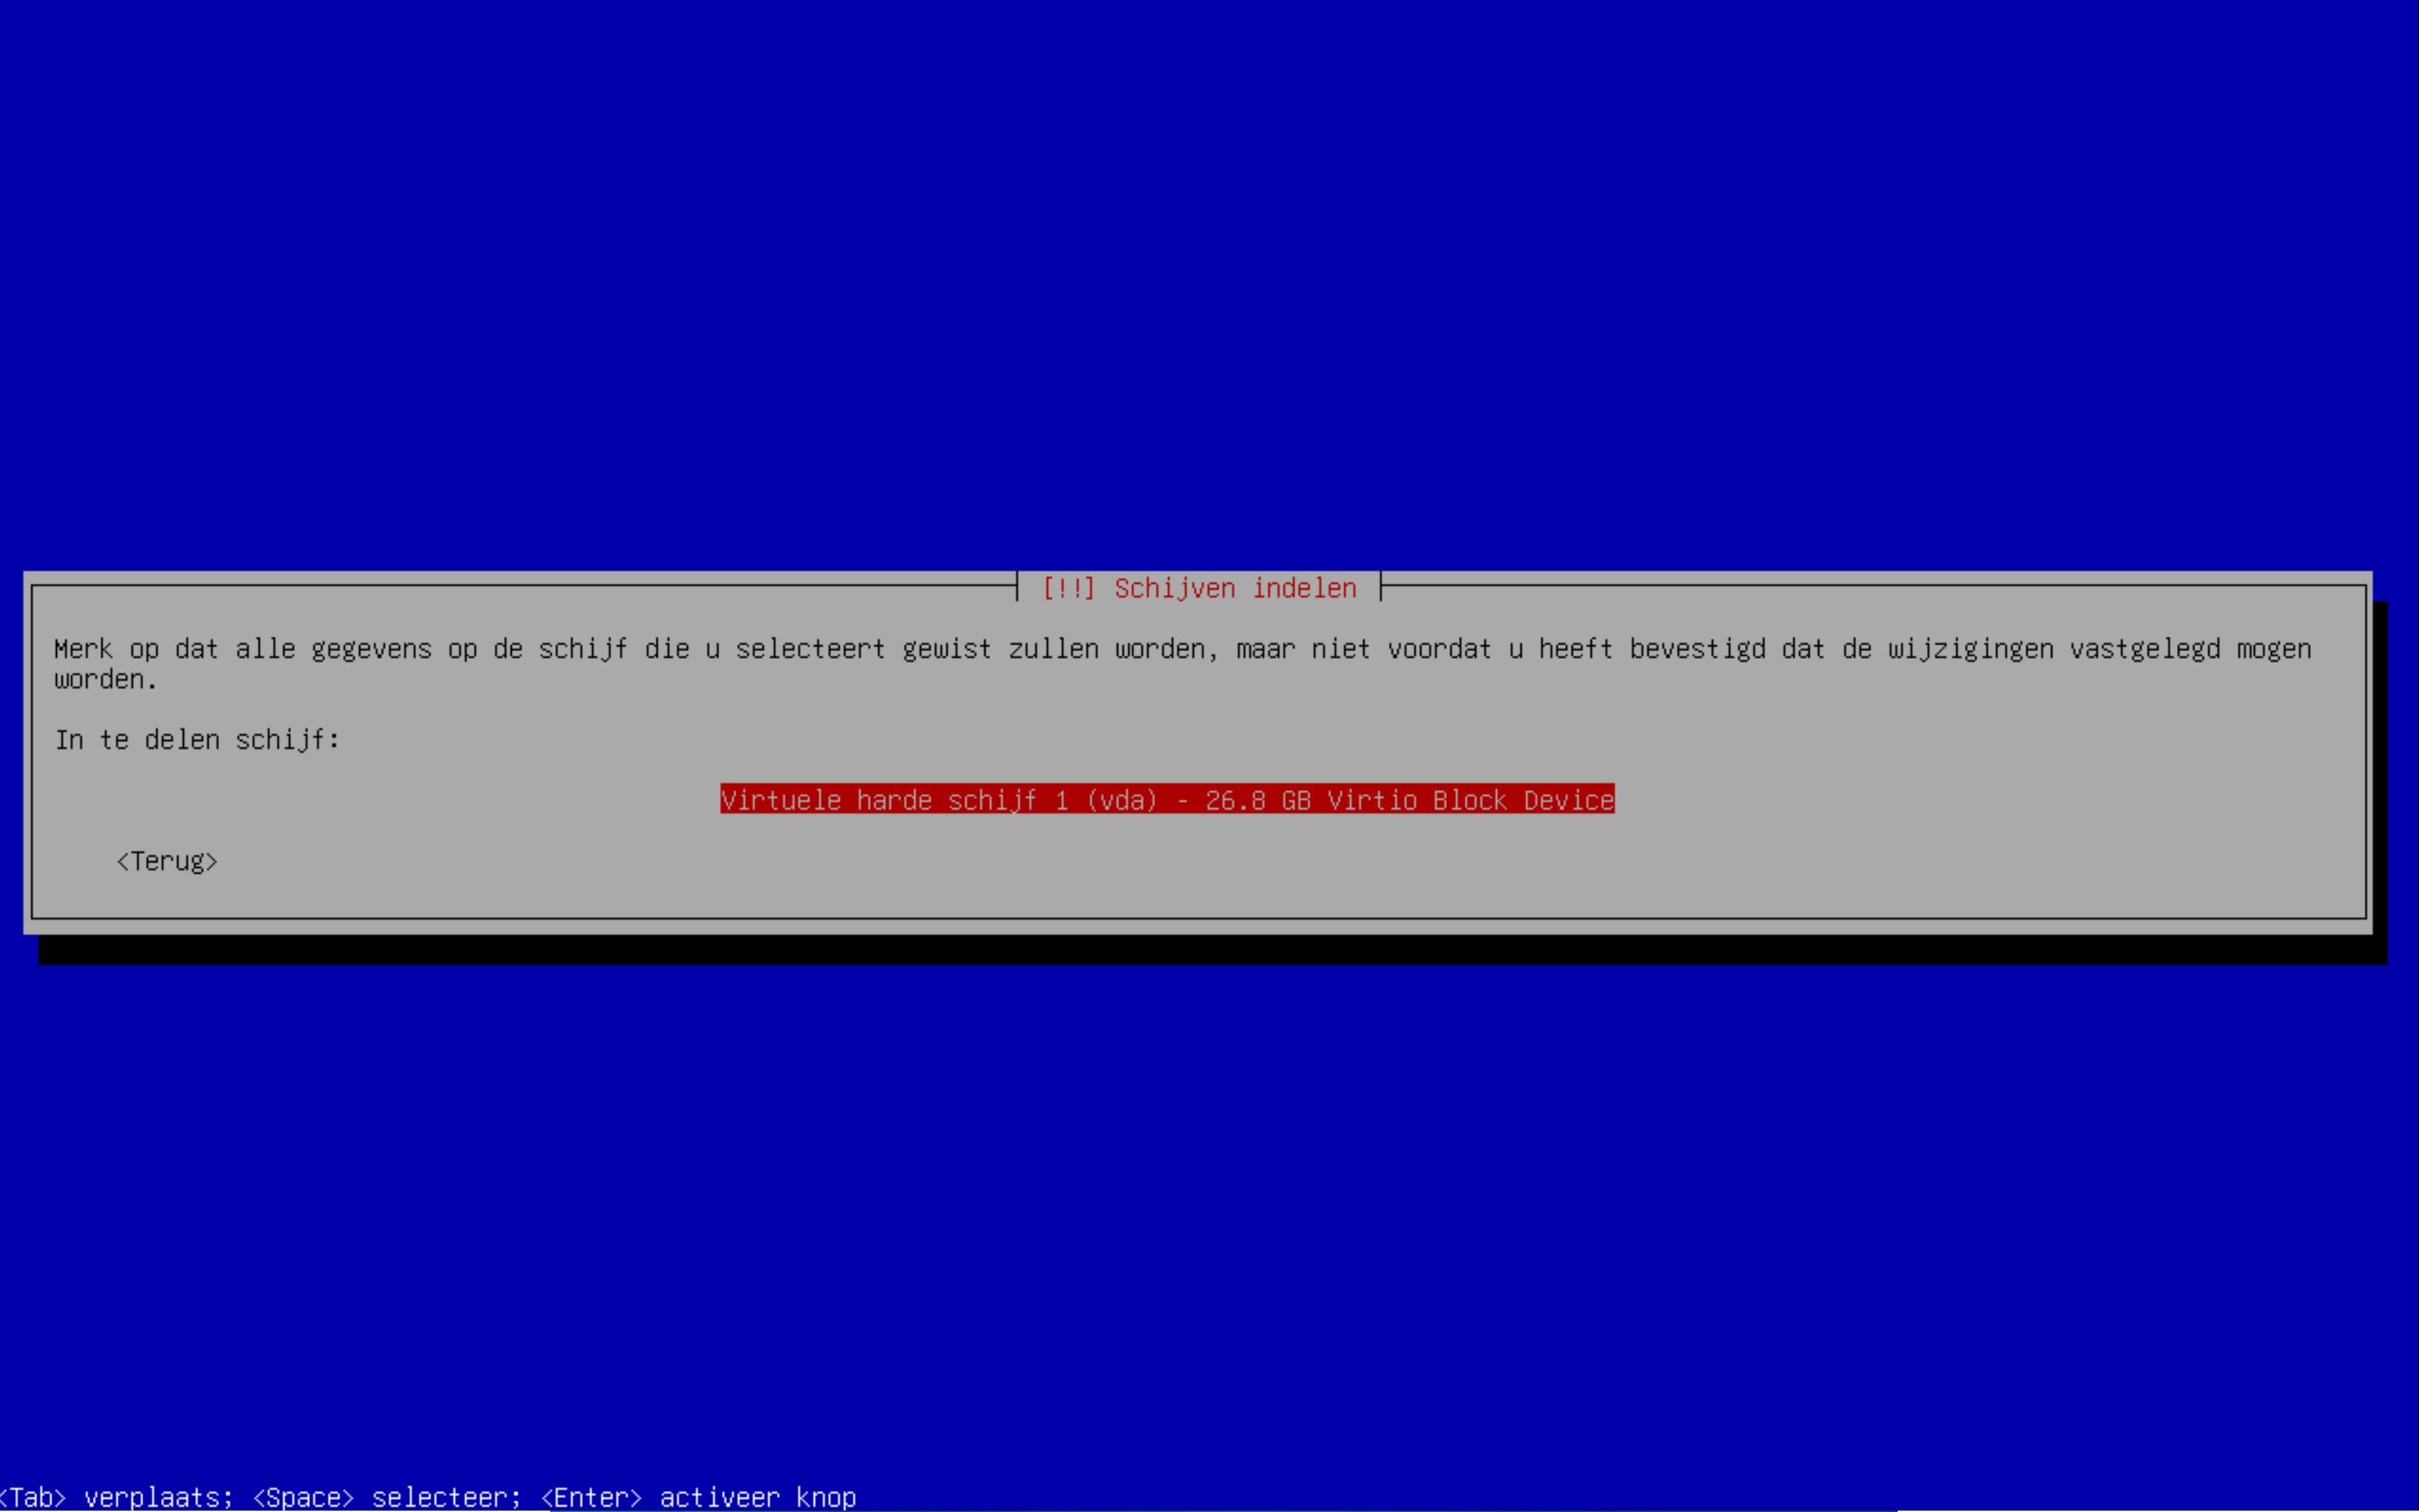
\includegraphics[width=\textwidth]{img/disk-kiezen.png}<1->
\end{frame}

\begin{frame}
   \frametitle{Disk indeling accepteren}
   \onslide<2>{\Enter op om door te gaan}
   \centering
   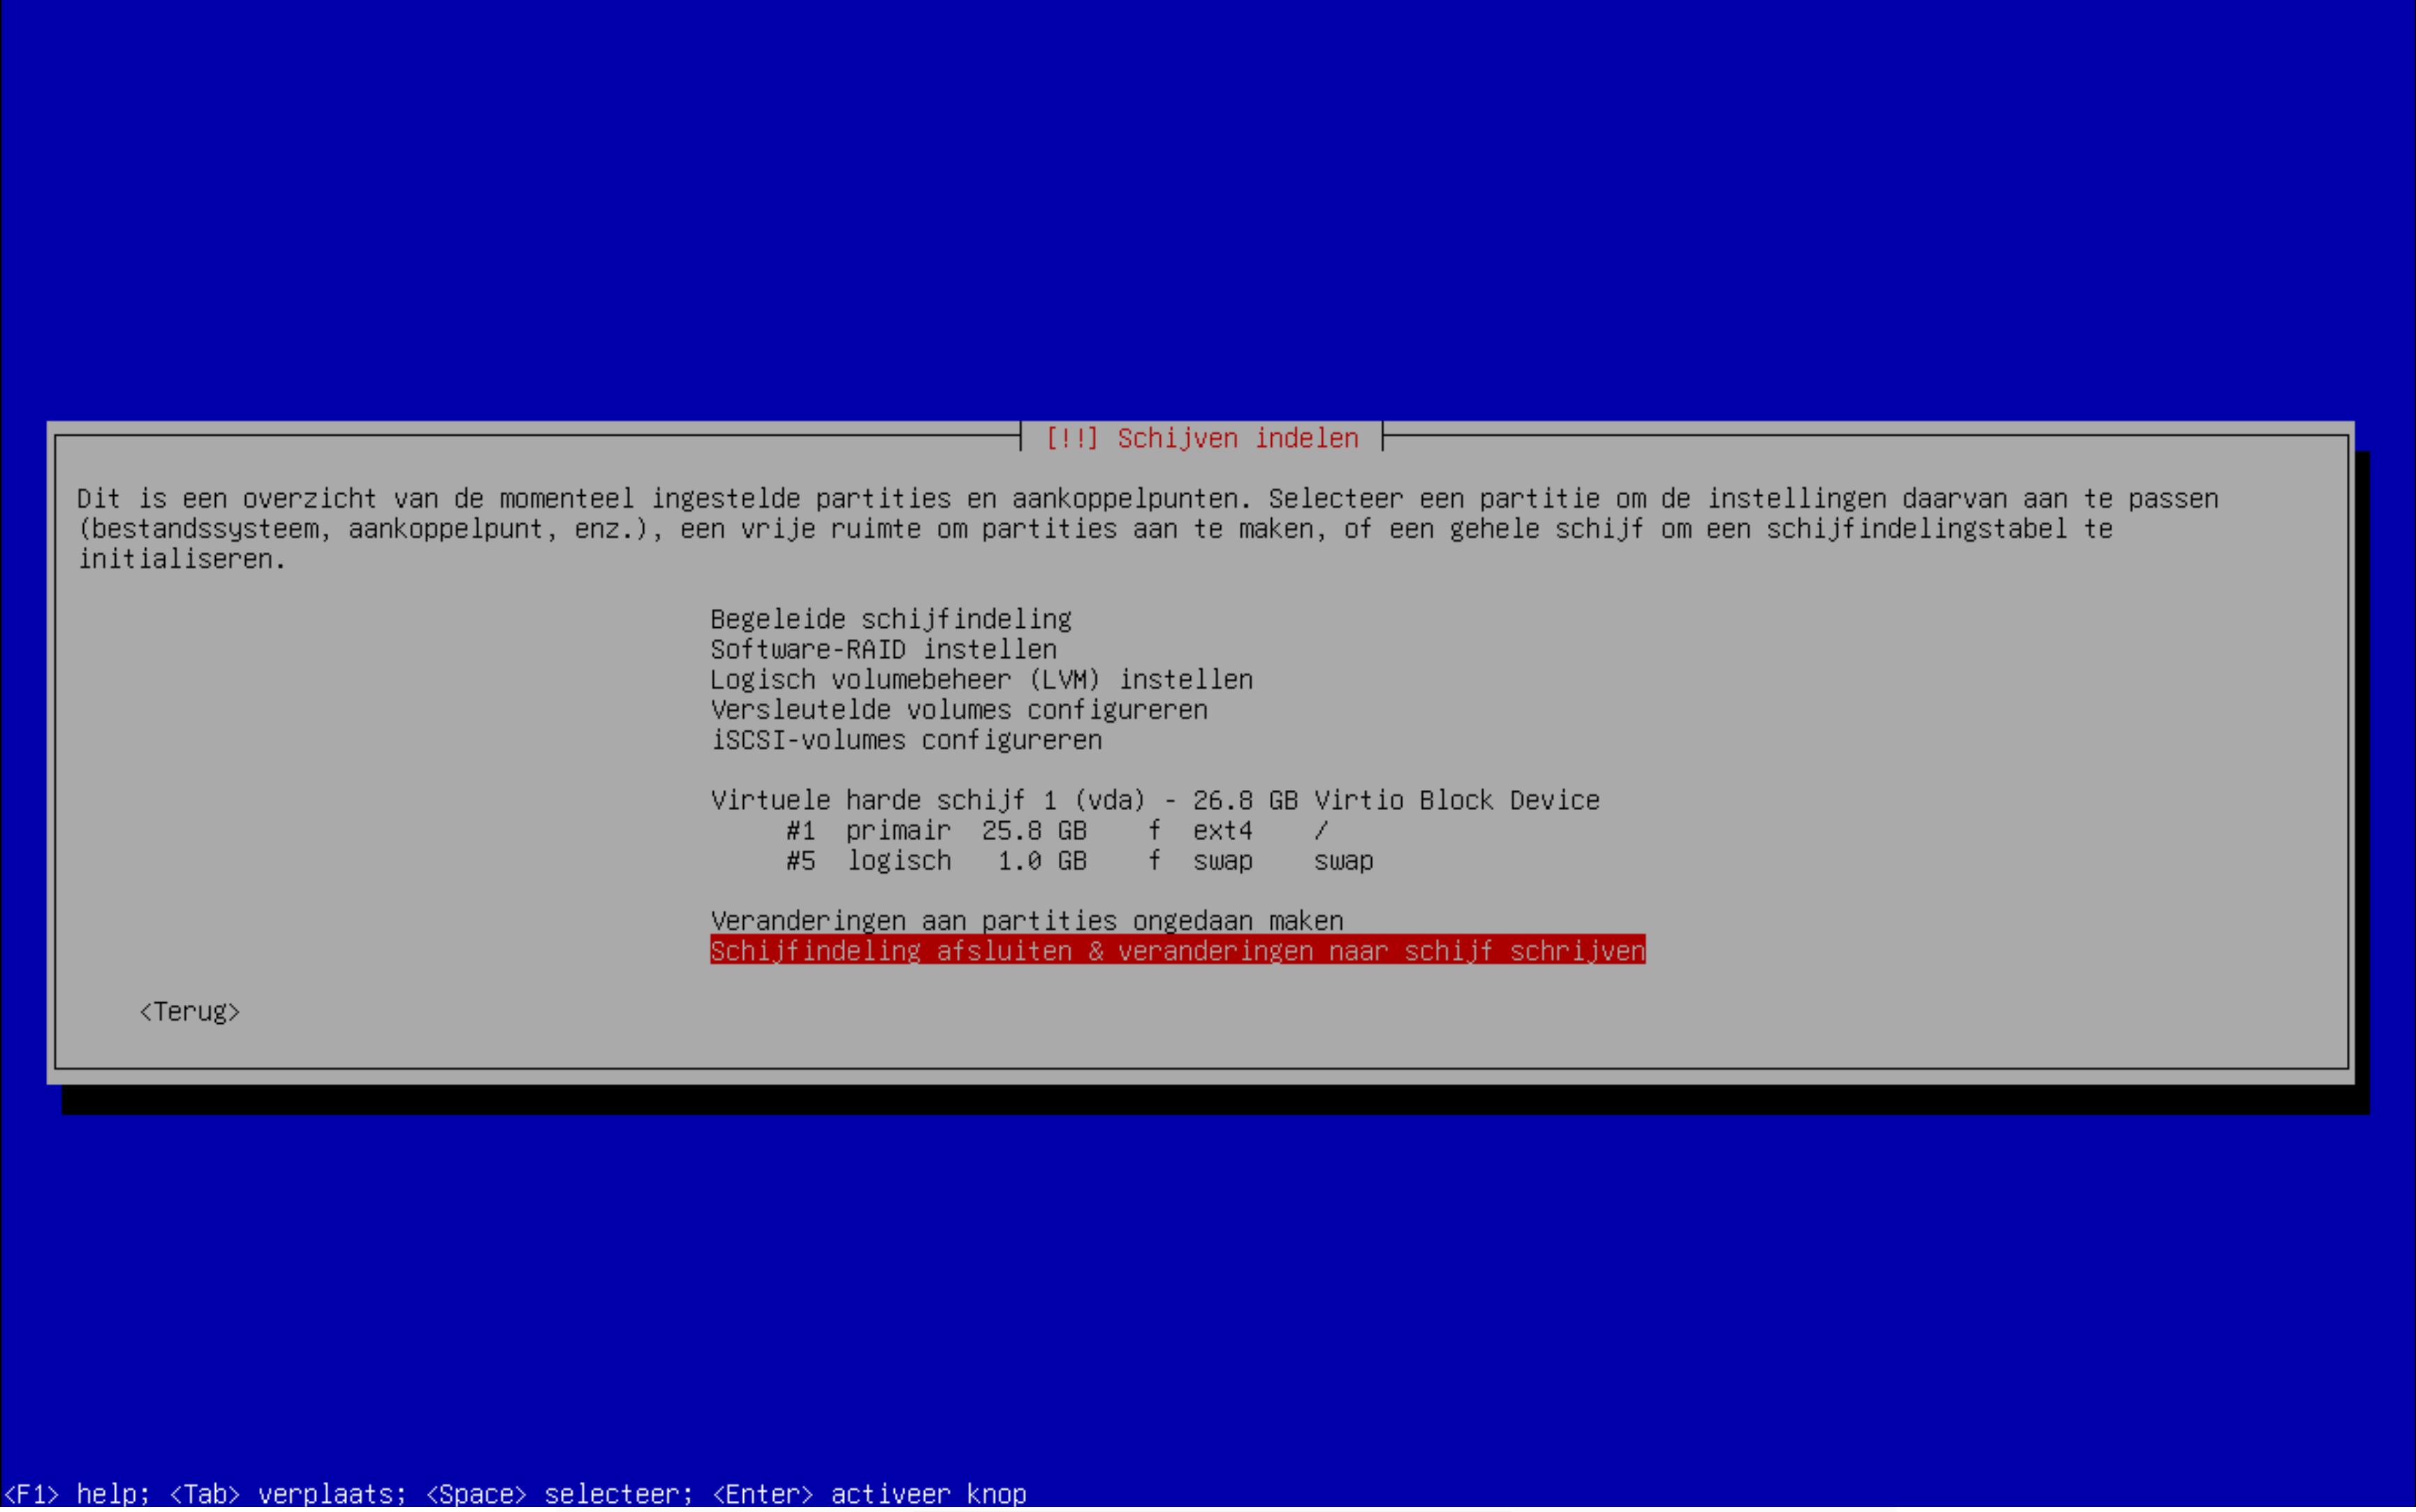
\includegraphics[width=\textwidth]{img/indeling-accepteren.png}<1->
\end{frame}

\begin{frame}
   \frametitle{Disk indeling bevestigen}
   \onslide<2->{\Tab om keuze op \texttt{<Ja>} te zetten, bevestig daarna met \Enter}
   
   \centering
   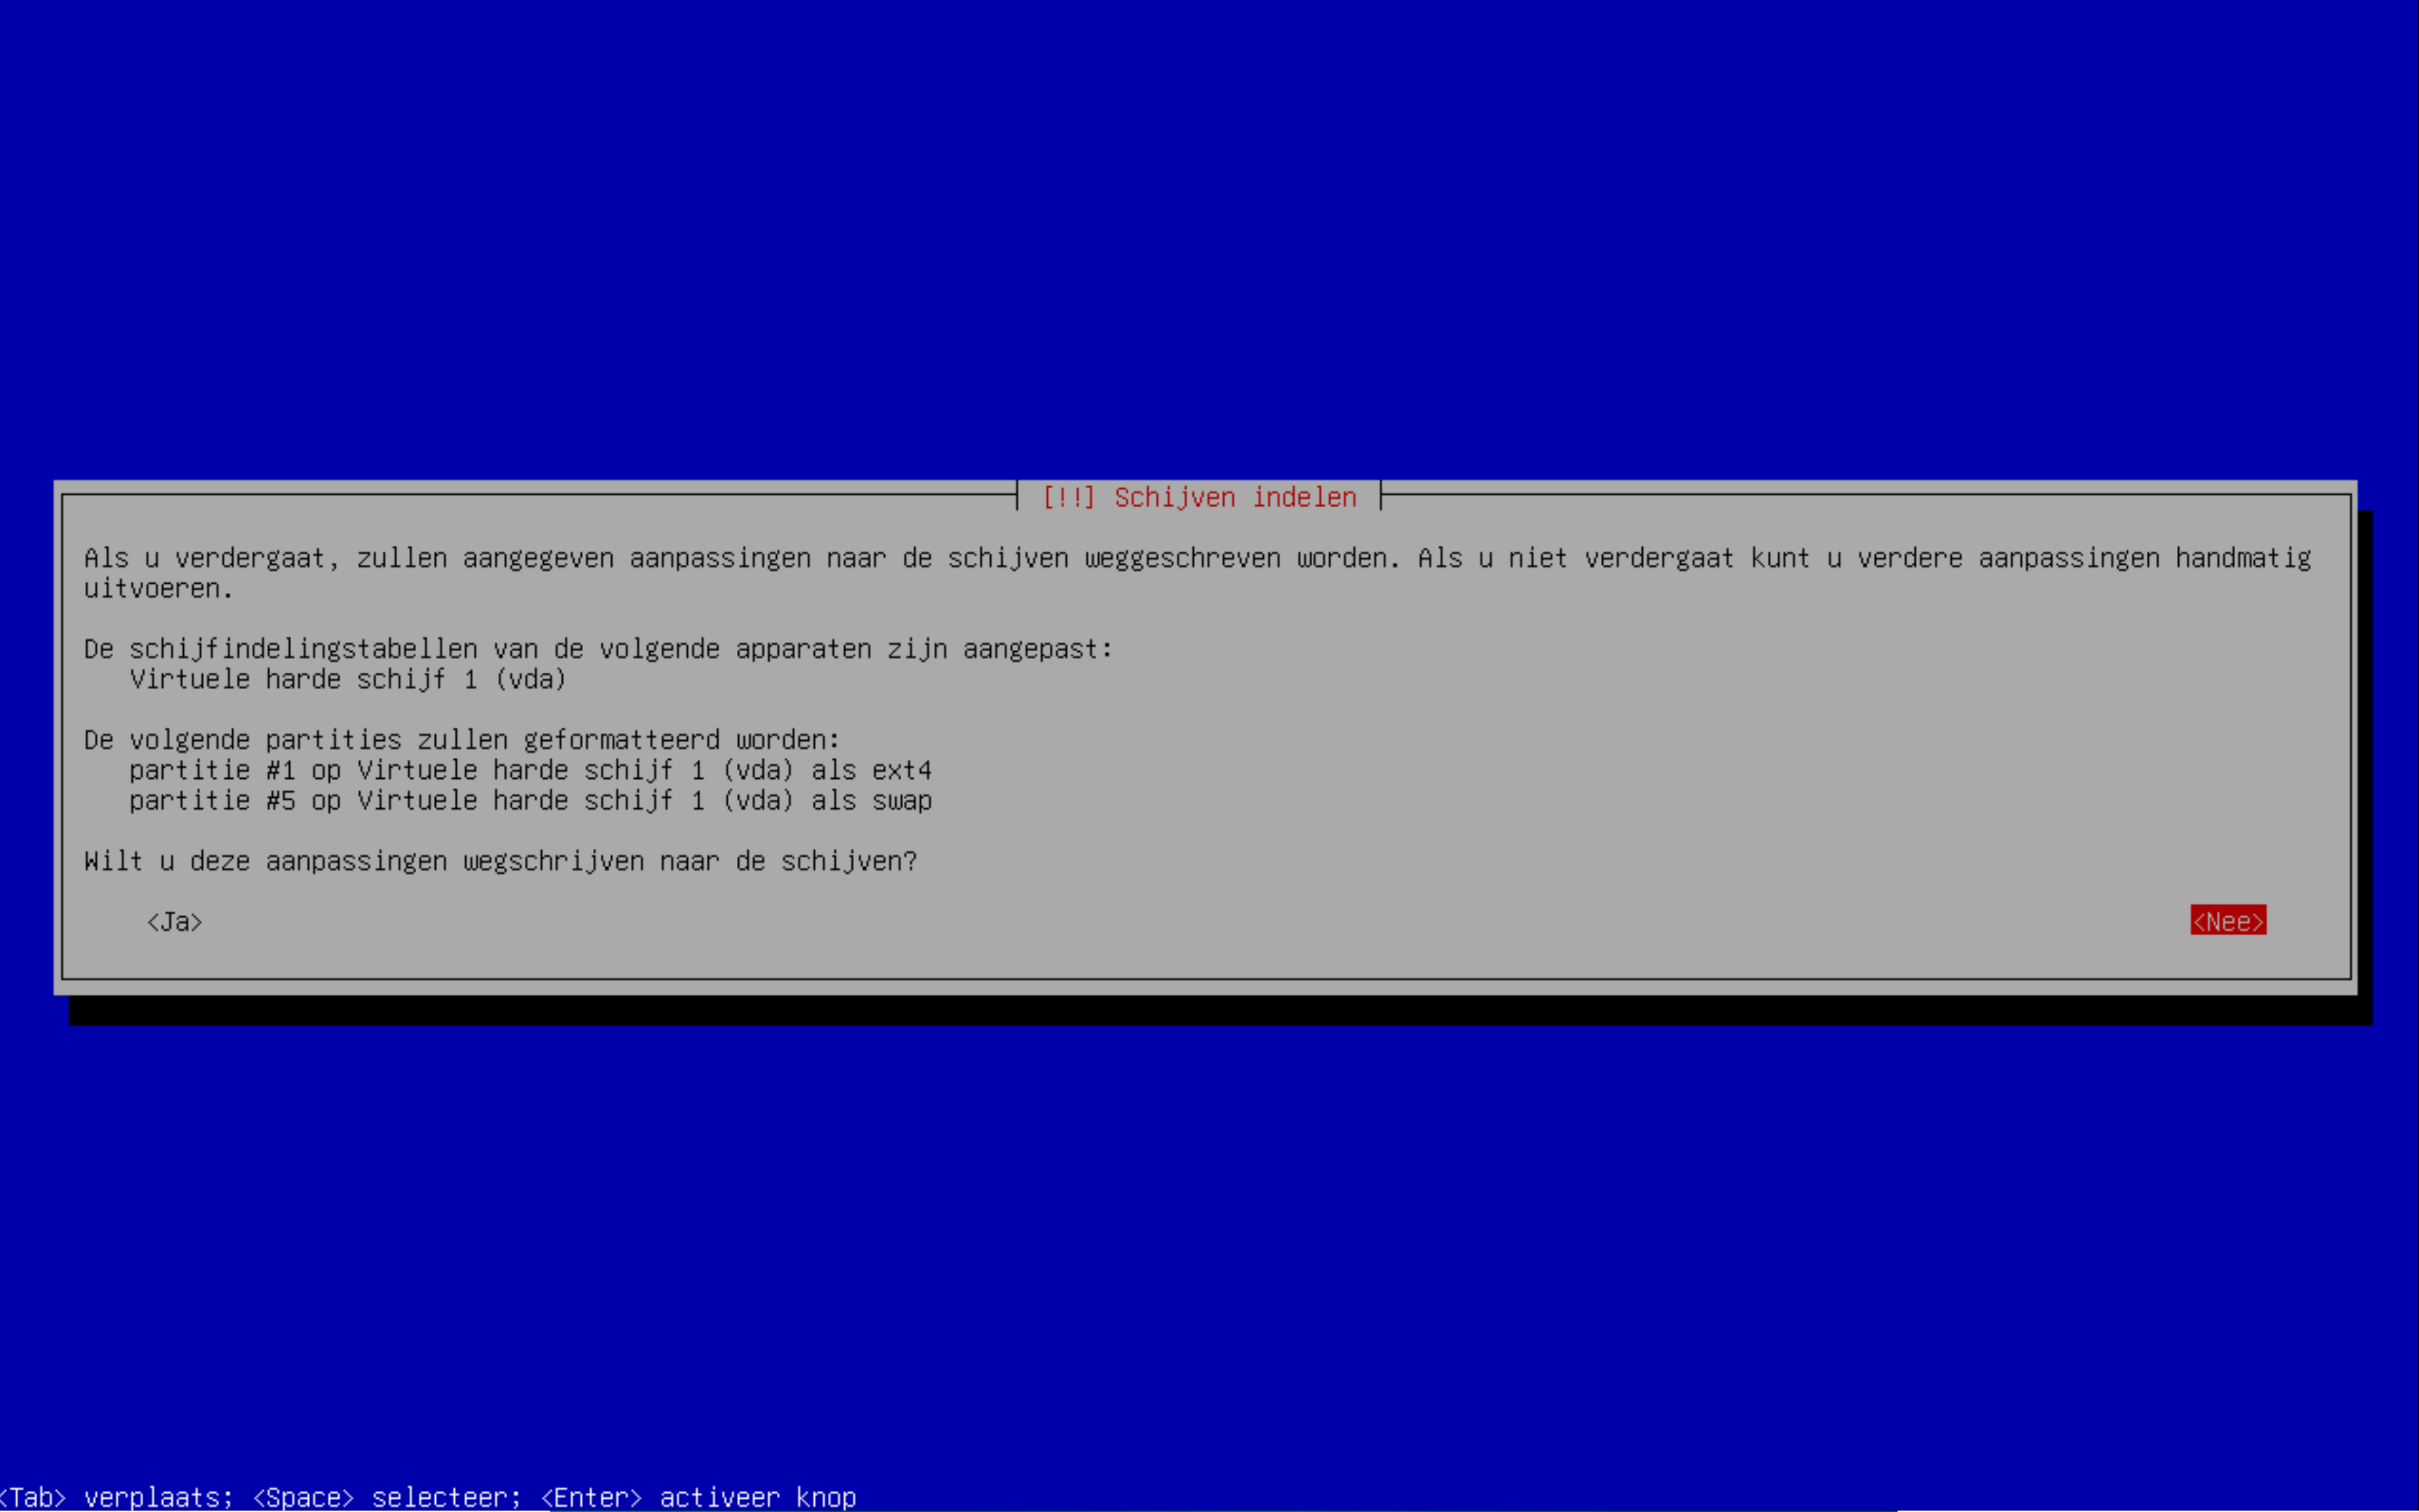
\includegraphics[width=\textwidth]{img/indeling-bevestigen.png}<1-2>
   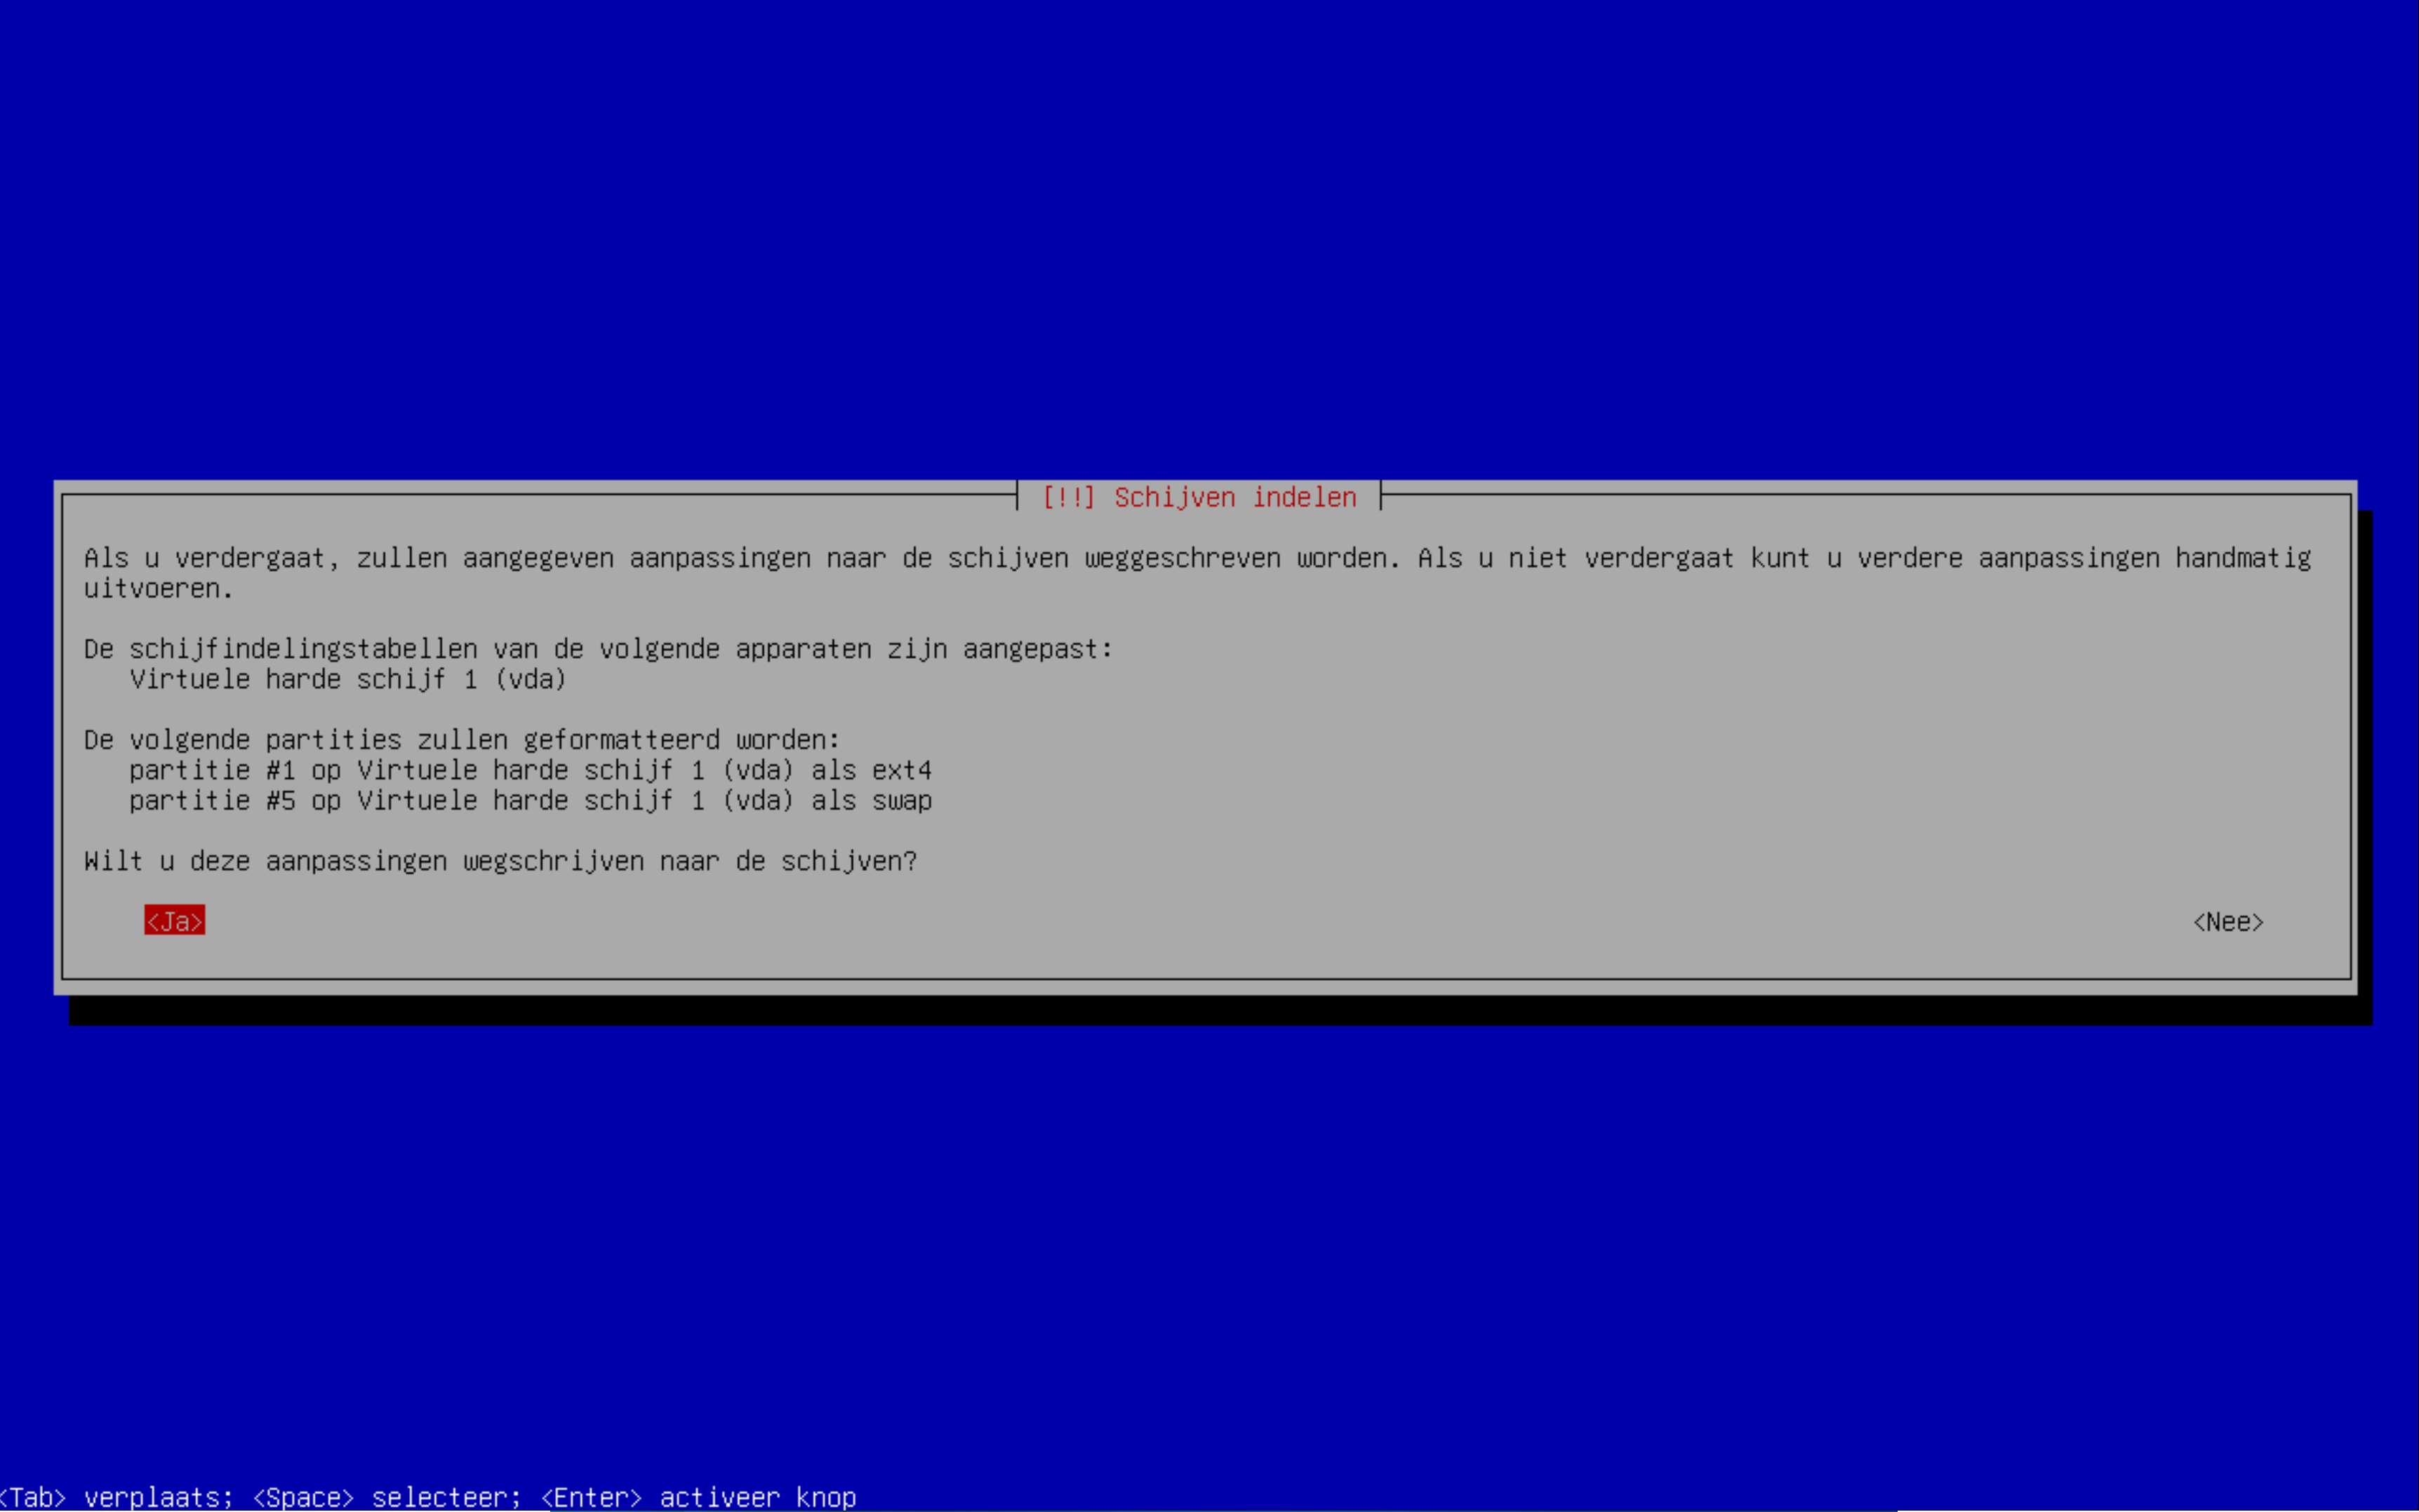
\includegraphics[width=\textwidth]{img/indeling-bevestigd.png}<3>
\end{frame}

\begin{frame}<beamer>
  \frametitle{Basissysteem}
   
   \centering
   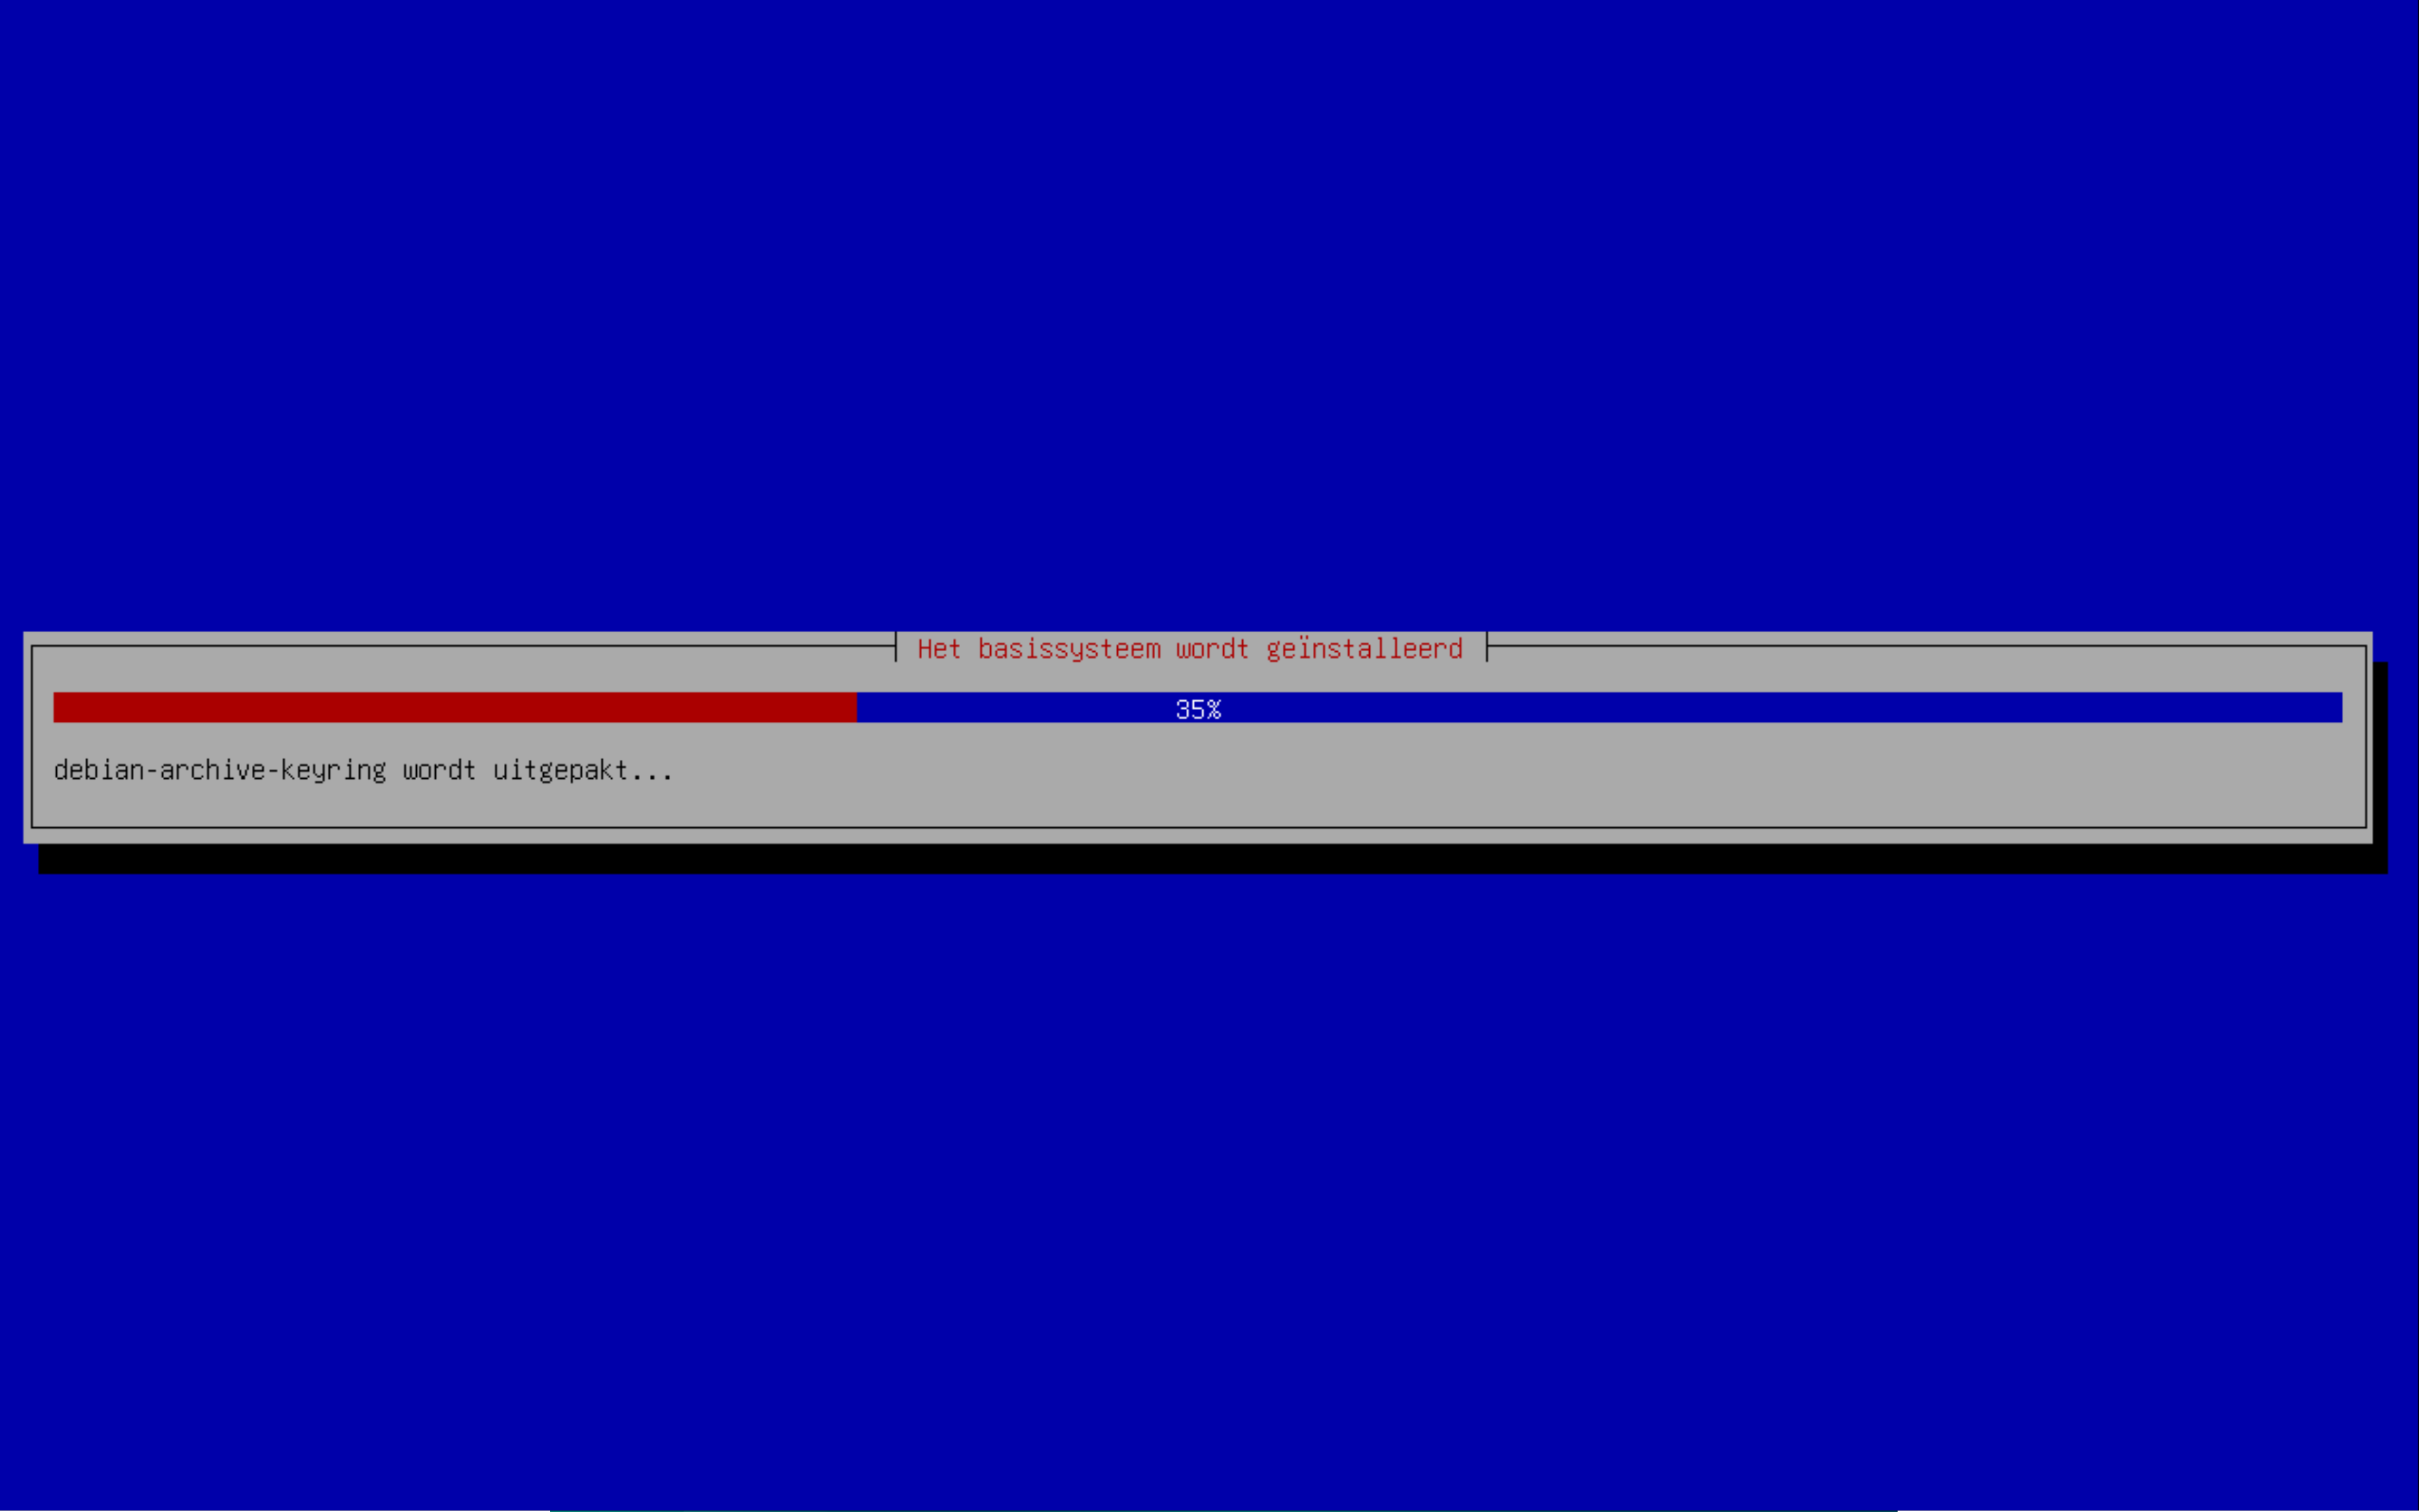
\includegraphics[width=\textwidth]{img/basissysteem.png}
\end{frame}

\begin{frame}<beamer>
  \frametitle{Programmatuur installeren}
   
   \centering
   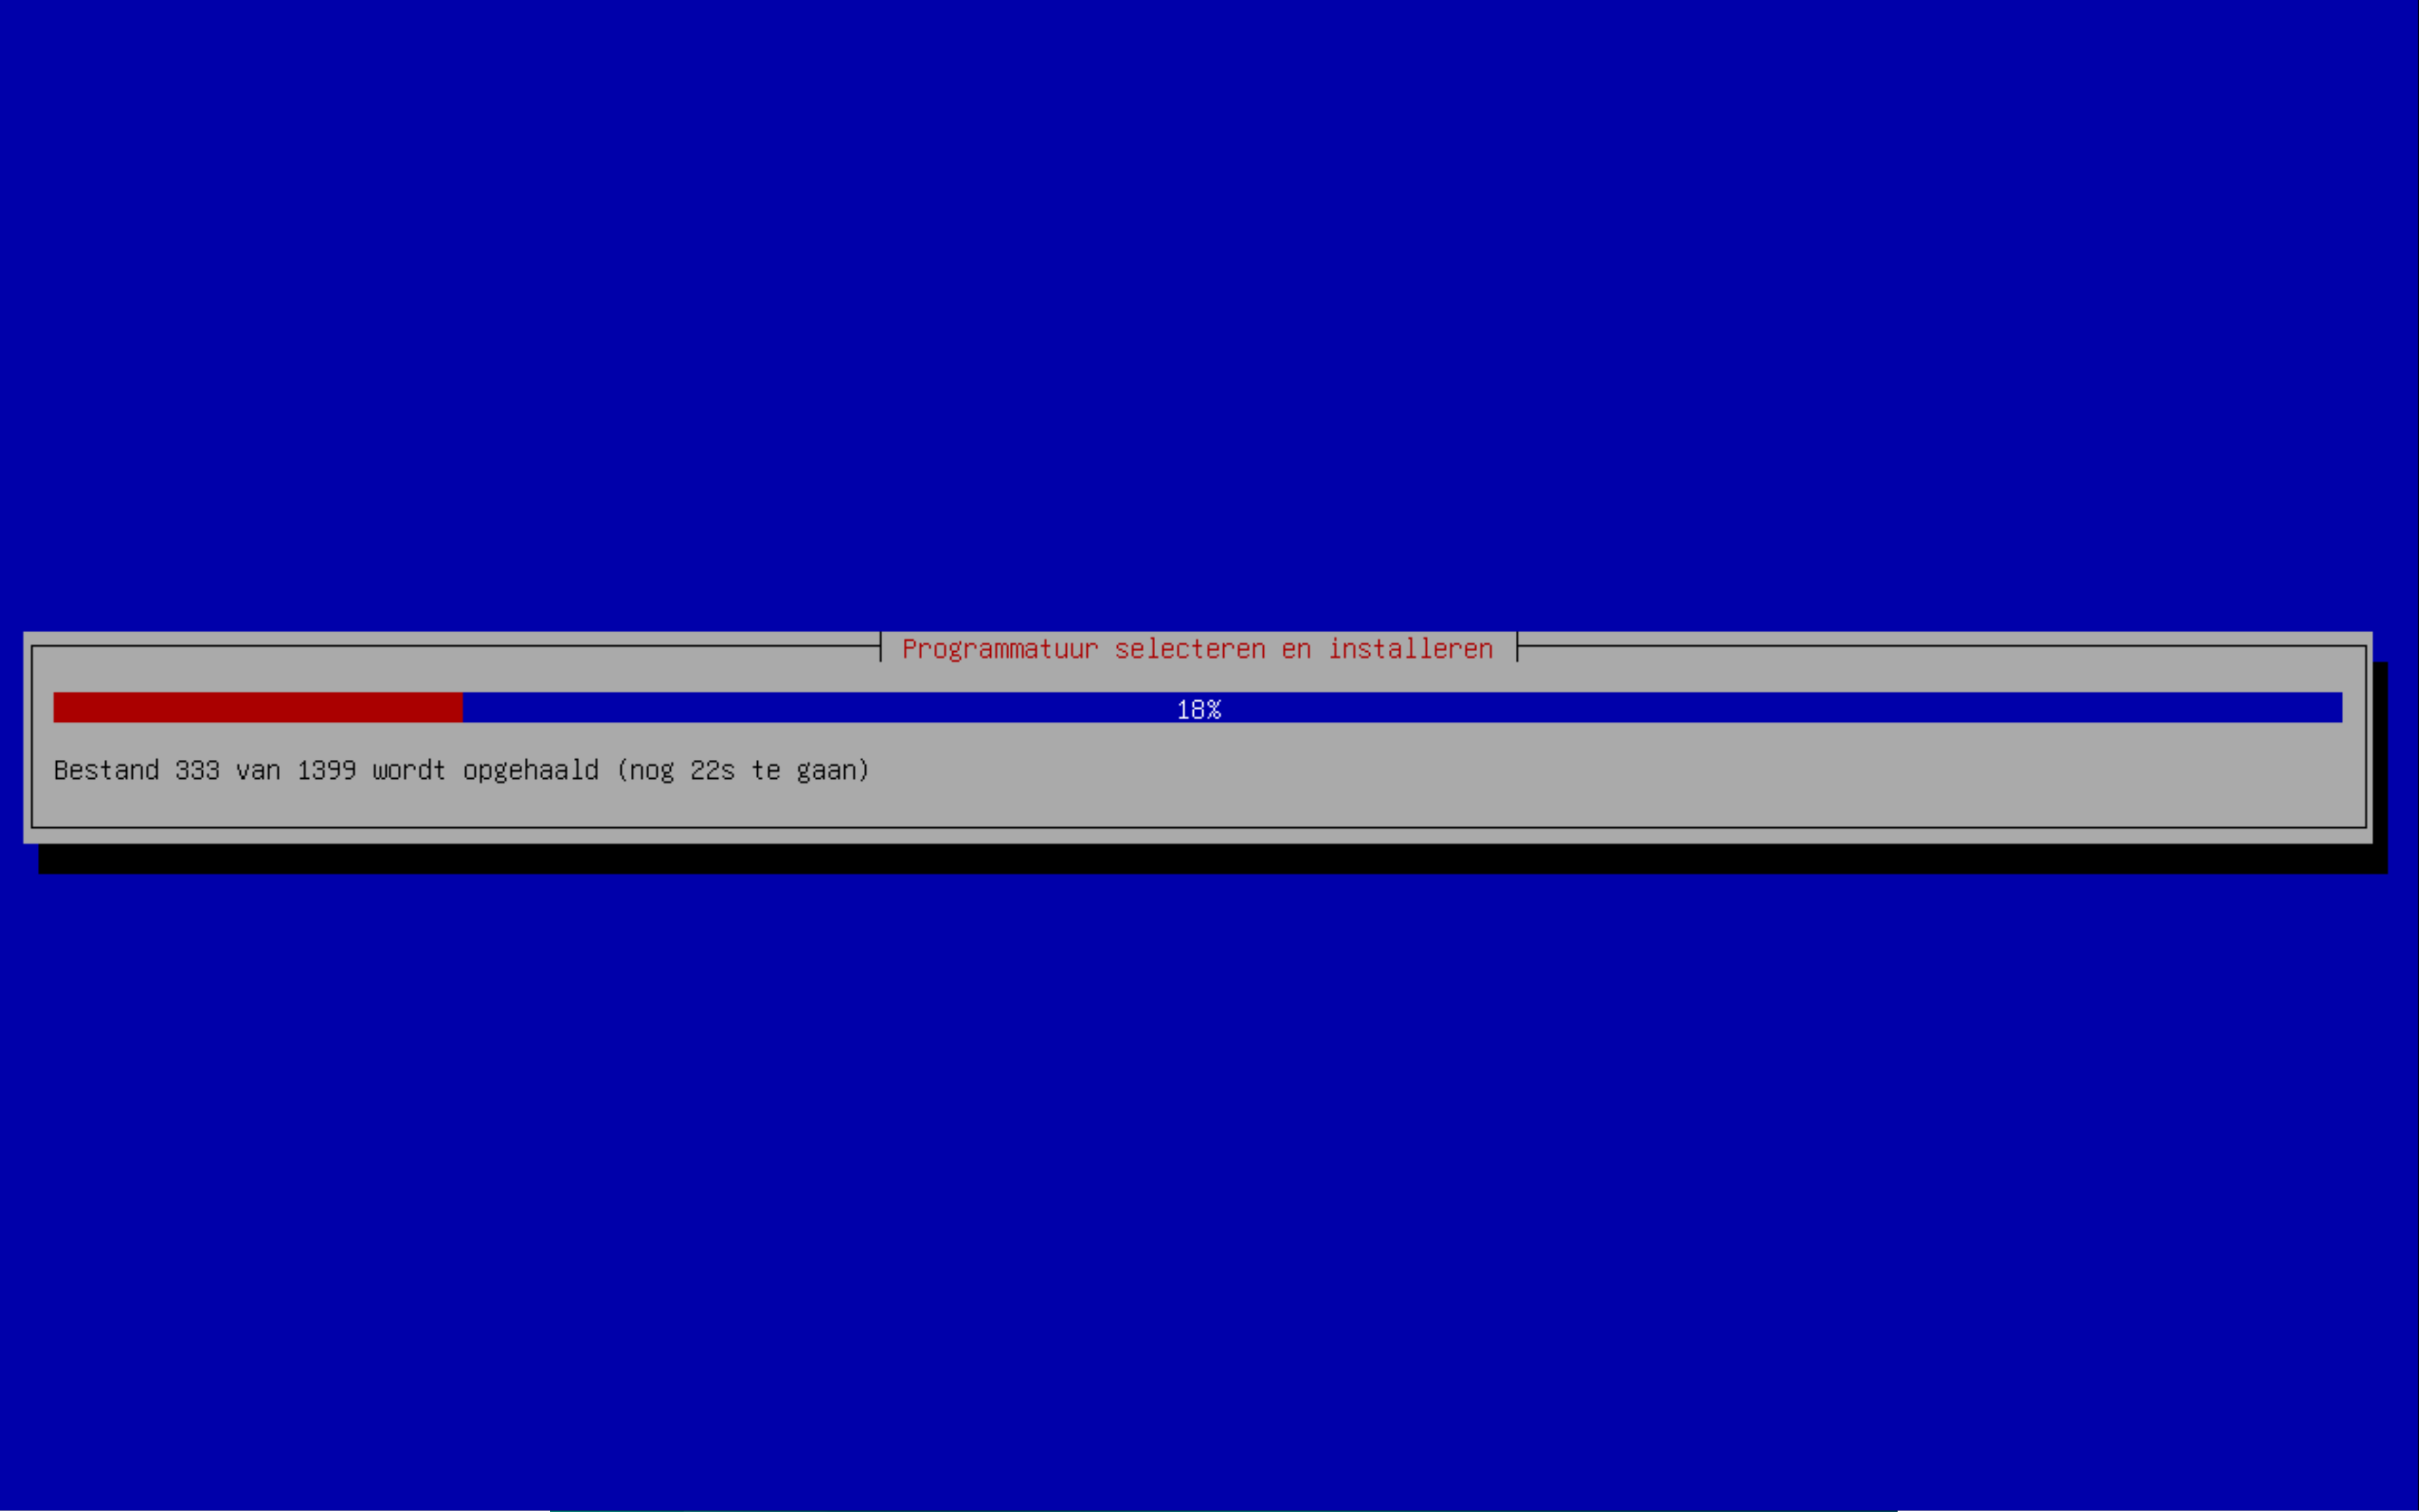
\includegraphics[width=\textwidth]{img/programmatuur.png}
\end{frame}

\begin{frame}<beamer>
  \frametitle{Preseed scripts}
   
   \centering
   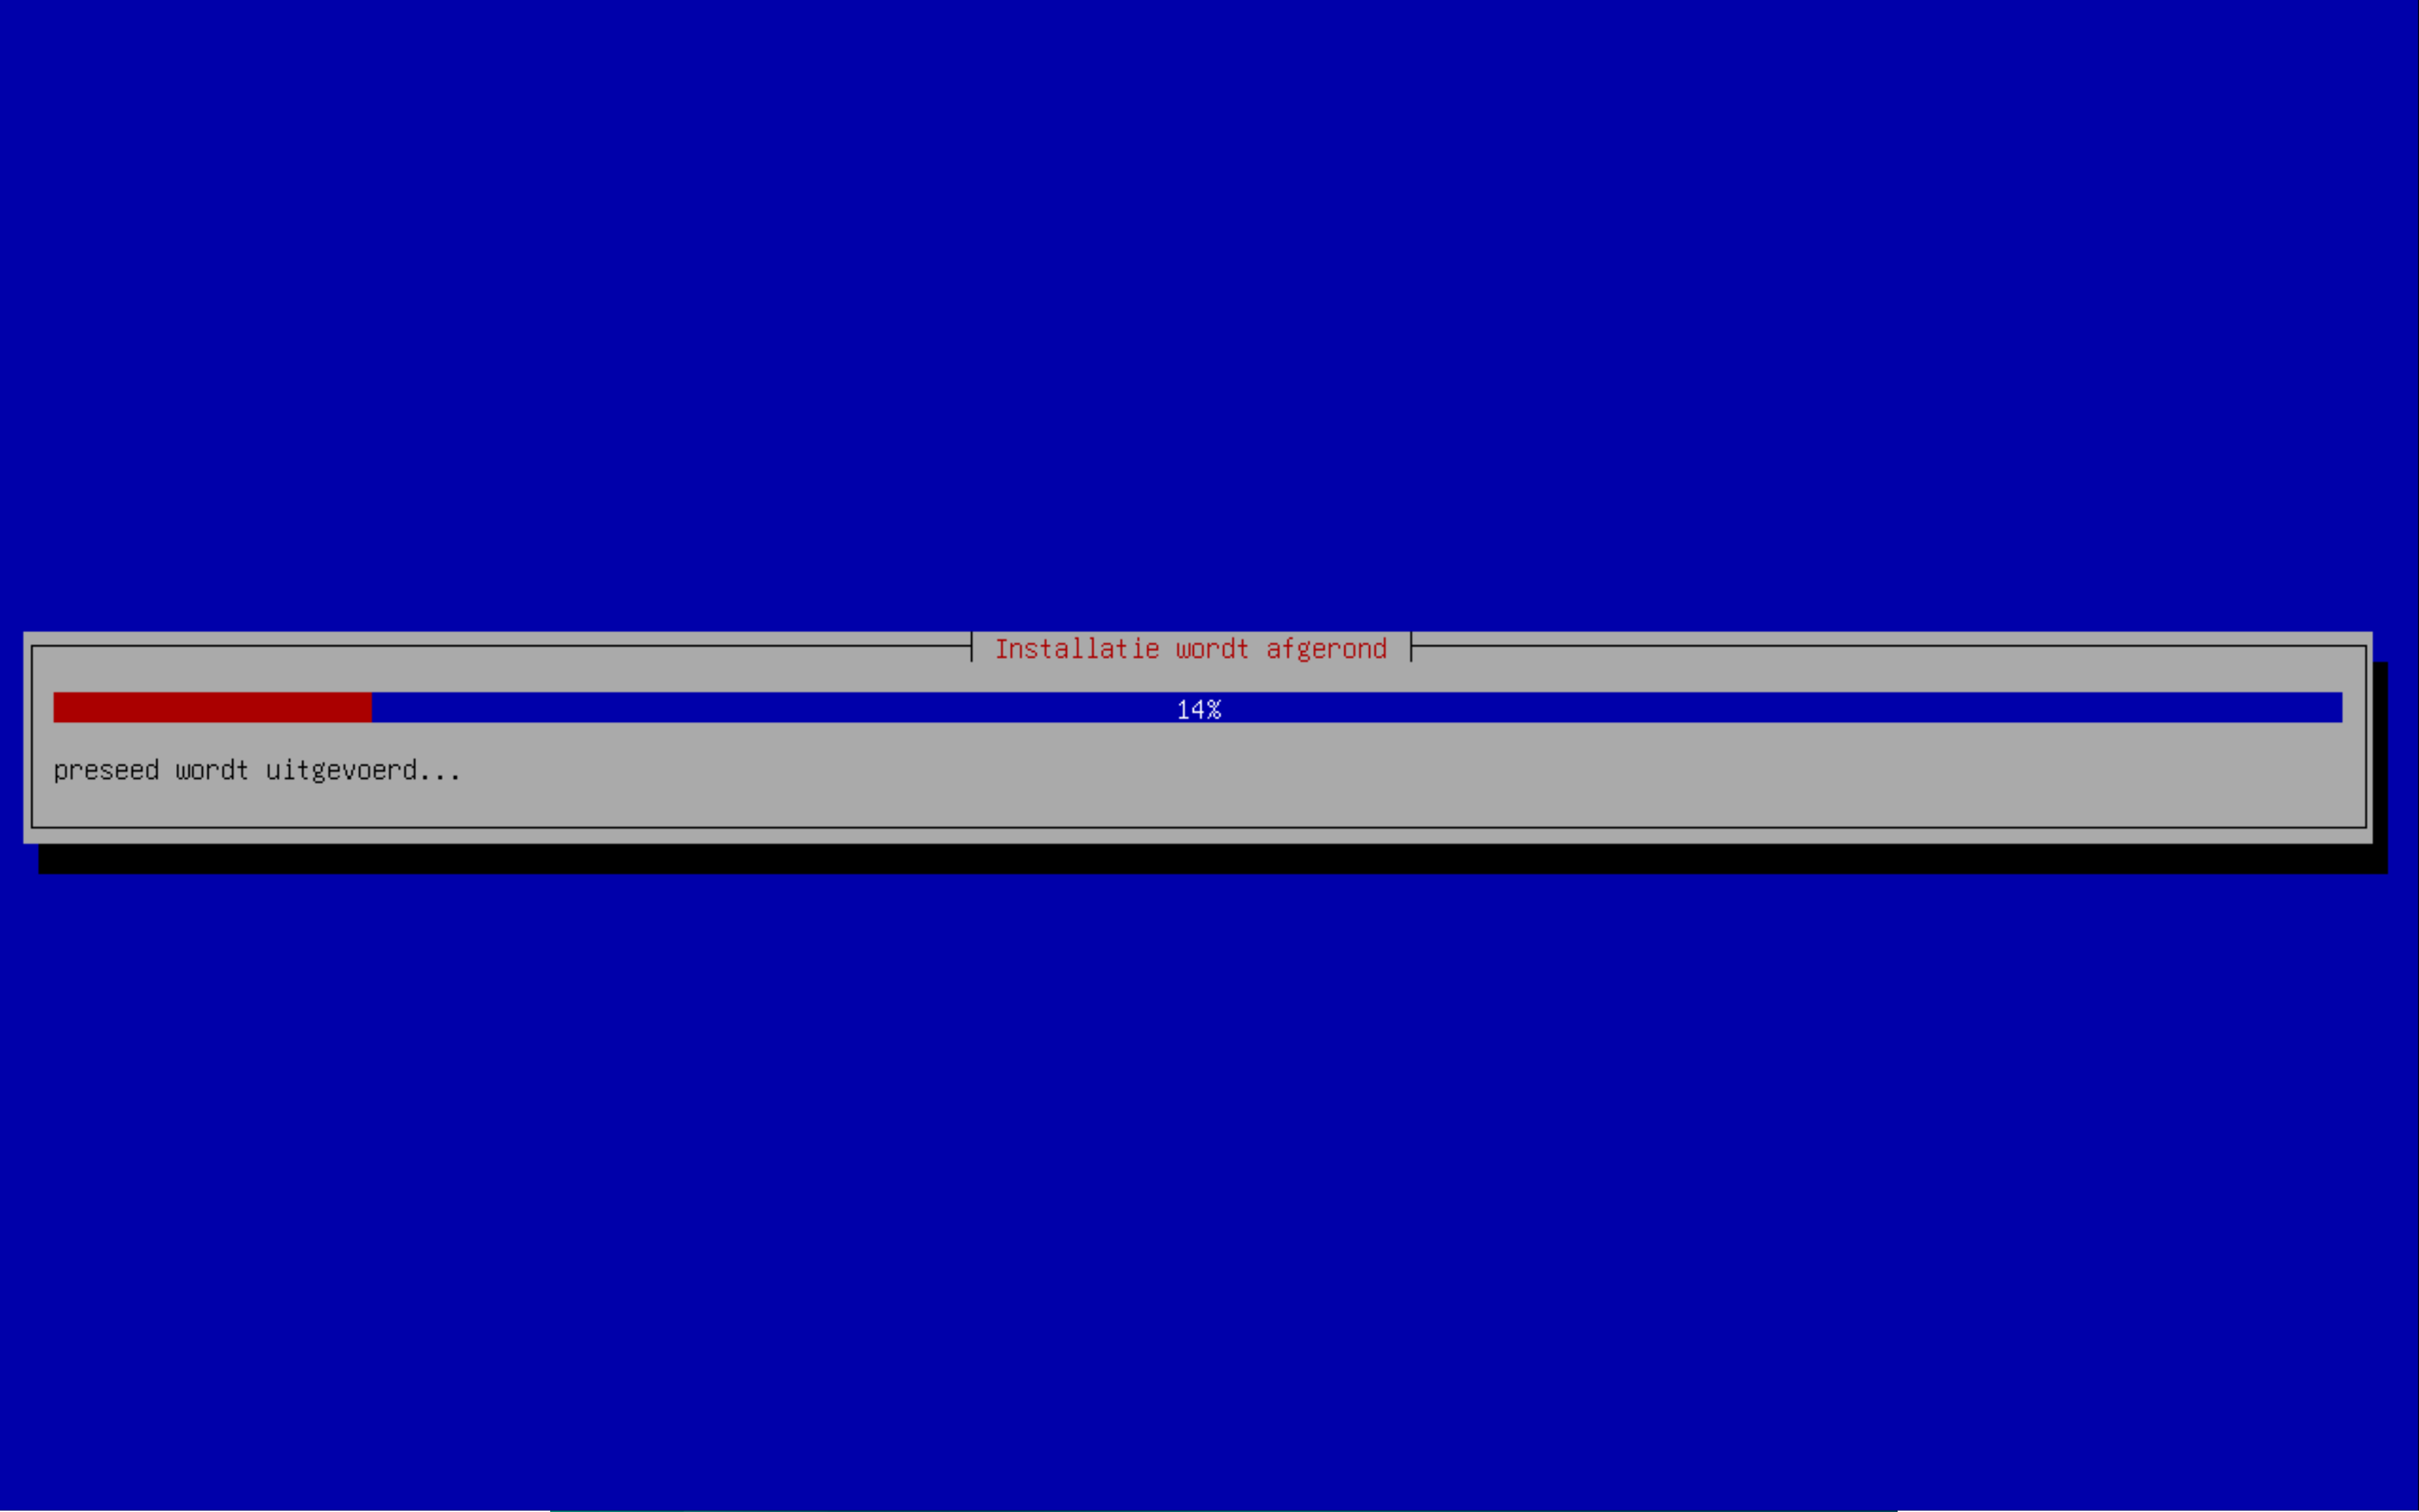
\includegraphics[width=\textwidth]{img/preseed.png}
\end{frame}

\subsection{Herstarten}

\begin{frame}
   \frametitle{Reboot na geslaagde installatie}
    \onslide<2>{Inloggen met \Enter dan als wachtwoord \texttt{tux} gevolgd door \Enter}
    \centering
    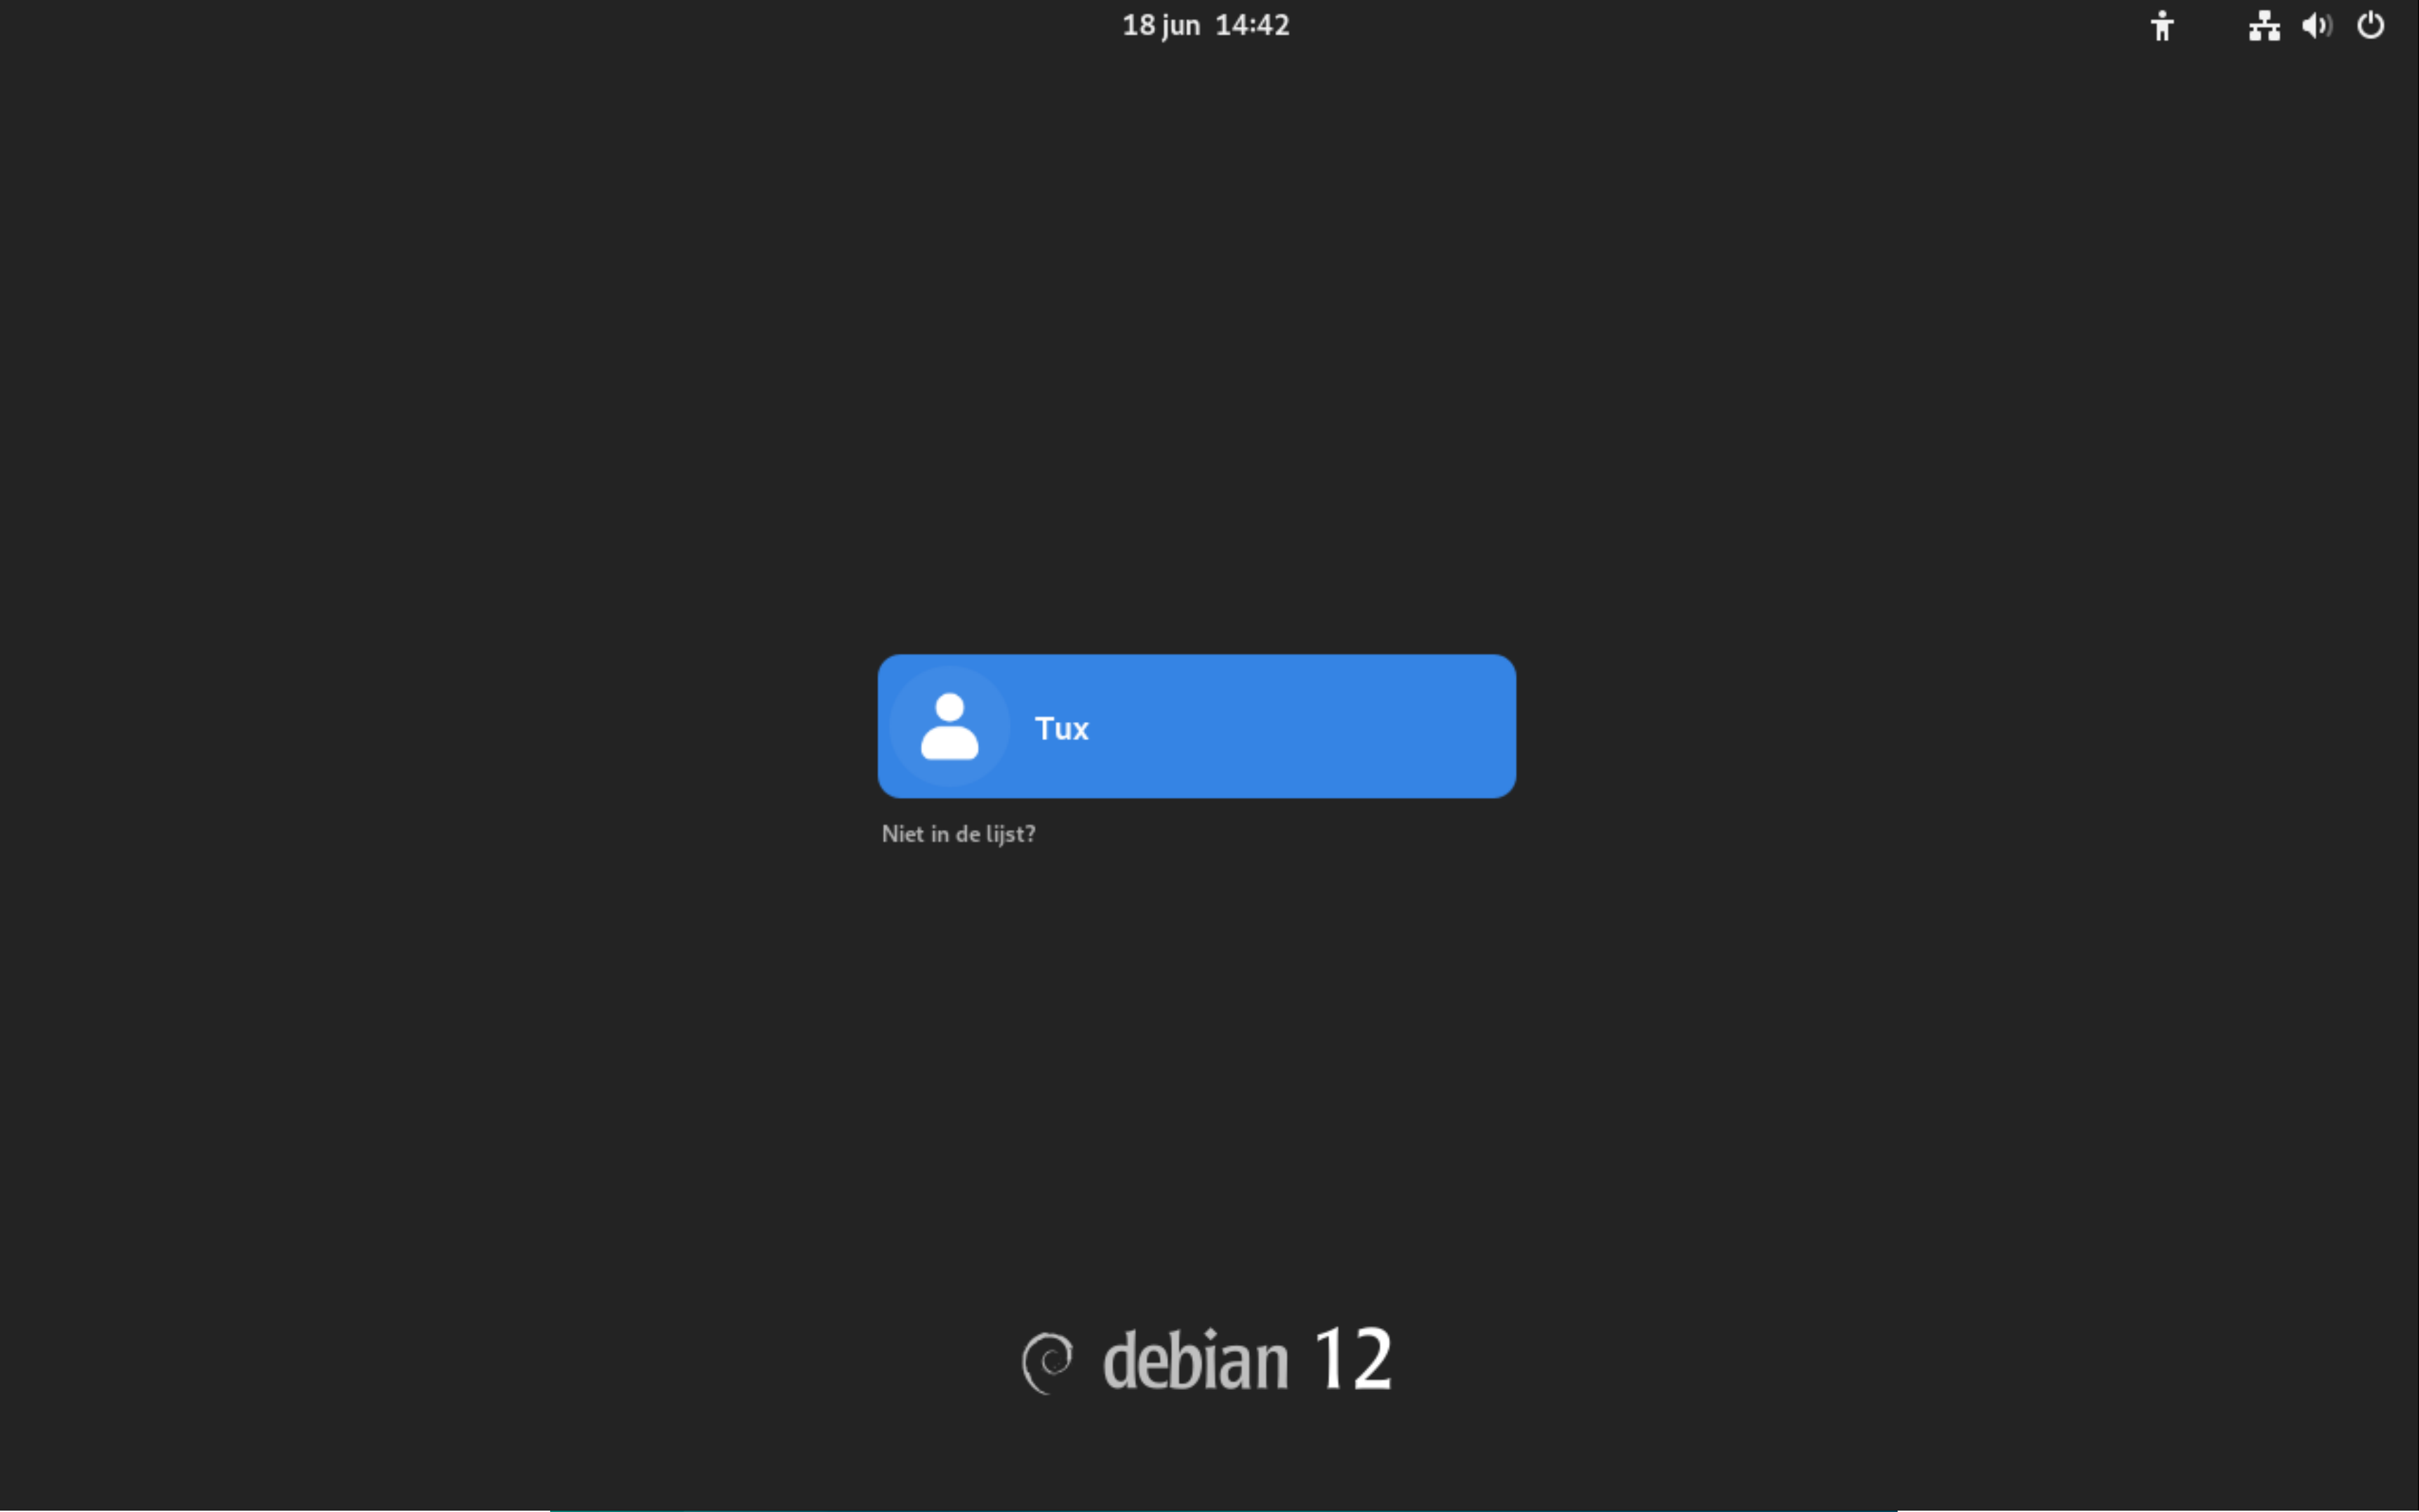
\includegraphics[width=\textwidth]{img/geslaagde-gnome-installatie.png}<1->
    
\end{frame}
%---------------------------------------------------------

\end{document}